\documentclass{article} % For LaTeX2e
\usepackage{iclr2025_conference,times}
\iclrfinalcopy

% Optional math commands from https://github.com/goodfeli/dlbook_notation.
%%%%% NEW MATH DEFINITIONS %%%%%

\usepackage{amsmath,amsfonts,bm}

% Mark sections of captions for referring to divisions of figures
\newcommand{\figleft}{{\em (Left)}}
\newcommand{\figcenter}{{\em (Center)}}
\newcommand{\figright}{{\em (Right)}}
\newcommand{\figtop}{{\em (Top)}}
\newcommand{\figbottom}{{\em (Bottom)}}
\newcommand{\captiona}{{\em (a)}}
\newcommand{\captionb}{{\em (b)}}
\newcommand{\captionc}{{\em (c)}}
\newcommand{\captiond}{{\em (d)}}

% Highlight a newly defined term
\newcommand{\newterm}[1]{{\bf #1}}


% Figure reference, lower-case.
\def\figref#1{figure~\ref{#1}}
% Figure reference, capital. For start of sentence
\def\Figref#1{Figure~\ref{#1}}
\def\twofigref#1#2{figures \ref{#1} and \ref{#2}}
\def\quadfigref#1#2#3#4{figures \ref{#1}, \ref{#2}, \ref{#3} and \ref{#4}}
% Section reference, lower-case.
\def\secref#1{section~\ref{#1}}
% Section reference, capital.
\def\Secref#1{Section~\ref{#1}}
% Reference to two sections.
\def\twosecrefs#1#2{sections \ref{#1} and \ref{#2}}
% Reference to three sections.
\def\secrefs#1#2#3{sections \ref{#1}, \ref{#2} and \ref{#3}}
% Reference to an equation, lower-case.
\def\eqref#1{equation~\ref{#1}}
% Reference to an equation, upper case
\def\Eqref#1{Equation~\ref{#1}}
% A raw reference to an equation---avoid using if possible
\def\plaineqref#1{\ref{#1}}
% Reference to a chapter, lower-case.
\def\chapref#1{chapter~\ref{#1}}
% Reference to an equation, upper case.
\def\Chapref#1{Chapter~\ref{#1}}
% Reference to a range of chapters
\def\rangechapref#1#2{chapters\ref{#1}--\ref{#2}}
% Reference to an algorithm, lower-case.
\def\algref#1{algorithm~\ref{#1}}
% Reference to an algorithm, upper case.
\def\Algref#1{Algorithm~\ref{#1}}
\def\twoalgref#1#2{algorithms \ref{#1} and \ref{#2}}
\def\Twoalgref#1#2{Algorithms \ref{#1} and \ref{#2}}
% Reference to a part, lower case
\def\partref#1{part~\ref{#1}}
% Reference to a part, upper case
\def\Partref#1{Part~\ref{#1}}
\def\twopartref#1#2{parts \ref{#1} and \ref{#2}}

\def\ceil#1{\lceil #1 \rceil}
\def\floor#1{\lfloor #1 \rfloor}
\def\1{\bm{1}}
\newcommand{\train}{\mathcal{D}}
\newcommand{\valid}{\mathcal{D_{\mathrm{valid}}}}
\newcommand{\test}{\mathcal{D_{\mathrm{test}}}}

\def\eps{{\epsilon}}


% Random variables
\def\reta{{\textnormal{$\eta$}}}
\def\ra{{\textnormal{a}}}
\def\rb{{\textnormal{b}}}
\def\rc{{\textnormal{c}}}
\def\rd{{\textnormal{d}}}
\def\re{{\textnormal{e}}}
\def\rf{{\textnormal{f}}}
\def\rg{{\textnormal{g}}}
\def\rh{{\textnormal{h}}}
\def\ri{{\textnormal{i}}}
\def\rj{{\textnormal{j}}}
\def\rk{{\textnormal{k}}}
\def\rl{{\textnormal{l}}}
% rm is already a command, just don't name any random variables m
\def\rn{{\textnormal{n}}}
\def\ro{{\textnormal{o}}}
\def\rp{{\textnormal{p}}}
\def\rq{{\textnormal{q}}}
\def\rr{{\textnormal{r}}}
\def\rs{{\textnormal{s}}}
\def\rt{{\textnormal{t}}}
\def\ru{{\textnormal{u}}}
\def\rv{{\textnormal{v}}}
\def\rw{{\textnormal{w}}}
\def\rx{{\textnormal{x}}}
\def\ry{{\textnormal{y}}}
\def\rz{{\textnormal{z}}}

% Random vectors
\def\rvepsilon{{\mathbf{\epsilon}}}
\def\rvtheta{{\mathbf{\theta}}}
\def\rva{{\mathbf{a}}}
\def\rvb{{\mathbf{b}}}
\def\rvc{{\mathbf{c}}}
\def\rvd{{\mathbf{d}}}
\def\rve{{\mathbf{e}}}
\def\rvf{{\mathbf{f}}}
\def\rvg{{\mathbf{g}}}
\def\rvh{{\mathbf{h}}}
\def\rvu{{\mathbf{i}}}
\def\rvj{{\mathbf{j}}}
\def\rvk{{\mathbf{k}}}
\def\rvl{{\mathbf{l}}}
\def\rvm{{\mathbf{m}}}
\def\rvn{{\mathbf{n}}}
\def\rvo{{\mathbf{o}}}
\def\rvp{{\mathbf{p}}}
\def\rvq{{\mathbf{q}}}
\def\rvr{{\mathbf{r}}}
\def\rvs{{\mathbf{s}}}
\def\rvt{{\mathbf{t}}}
\def\rvu{{\mathbf{u}}}
\def\rvv{{\mathbf{v}}}
\def\rvw{{\mathbf{w}}}
\def\rvx{{\mathbf{x}}}
\def\rvy{{\mathbf{y}}}
\def\rvz{{\mathbf{z}}}

% Elements of random vectors
\def\erva{{\textnormal{a}}}
\def\ervb{{\textnormal{b}}}
\def\ervc{{\textnormal{c}}}
\def\ervd{{\textnormal{d}}}
\def\erve{{\textnormal{e}}}
\def\ervf{{\textnormal{f}}}
\def\ervg{{\textnormal{g}}}
\def\ervh{{\textnormal{h}}}
\def\ervi{{\textnormal{i}}}
\def\ervj{{\textnormal{j}}}
\def\ervk{{\textnormal{k}}}
\def\ervl{{\textnormal{l}}}
\def\ervm{{\textnormal{m}}}
\def\ervn{{\textnormal{n}}}
\def\ervo{{\textnormal{o}}}
\def\ervp{{\textnormal{p}}}
\def\ervq{{\textnormal{q}}}
\def\ervr{{\textnormal{r}}}
\def\ervs{{\textnormal{s}}}
\def\ervt{{\textnormal{t}}}
\def\ervu{{\textnormal{u}}}
\def\ervv{{\textnormal{v}}}
\def\ervw{{\textnormal{w}}}
\def\ervx{{\textnormal{x}}}
\def\ervy{{\textnormal{y}}}
\def\ervz{{\textnormal{z}}}

% Random matrices
\def\rmA{{\mathbf{A}}}
\def\rmB{{\mathbf{B}}}
\def\rmC{{\mathbf{C}}}
\def\rmD{{\mathbf{D}}}
\def\rmE{{\mathbf{E}}}
\def\rmF{{\mathbf{F}}}
\def\rmG{{\mathbf{G}}}
\def\rmH{{\mathbf{H}}}
\def\rmI{{\mathbf{I}}}
\def\rmJ{{\mathbf{J}}}
\def\rmK{{\mathbf{K}}}
\def\rmL{{\mathbf{L}}}
\def\rmM{{\mathbf{M}}}
\def\rmN{{\mathbf{N}}}
\def\rmO{{\mathbf{O}}}
\def\rmP{{\mathbf{P}}}
\def\rmQ{{\mathbf{Q}}}
\def\rmR{{\mathbf{R}}}
\def\rmS{{\mathbf{S}}}
\def\rmT{{\mathbf{T}}}
\def\rmU{{\mathbf{U}}}
\def\rmV{{\mathbf{V}}}
\def\rmW{{\mathbf{W}}}
\def\rmX{{\mathbf{X}}}
\def\rmY{{\mathbf{Y}}}
\def\rmZ{{\mathbf{Z}}}

% Elements of random matrices
\def\ermA{{\textnormal{A}}}
\def\ermB{{\textnormal{B}}}
\def\ermC{{\textnormal{C}}}
\def\ermD{{\textnormal{D}}}
\def\ermE{{\textnormal{E}}}
\def\ermF{{\textnormal{F}}}
\def\ermG{{\textnormal{G}}}
\def\ermH{{\textnormal{H}}}
\def\ermI{{\textnormal{I}}}
\def\ermJ{{\textnormal{J}}}
\def\ermK{{\textnormal{K}}}
\def\ermL{{\textnormal{L}}}
\def\ermM{{\textnormal{M}}}
\def\ermN{{\textnormal{N}}}
\def\ermO{{\textnormal{O}}}
\def\ermP{{\textnormal{P}}}
\def\ermQ{{\textnormal{Q}}}
\def\ermR{{\textnormal{R}}}
\def\ermS{{\textnormal{S}}}
\def\ermT{{\textnormal{T}}}
\def\ermU{{\textnormal{U}}}
\def\ermV{{\textnormal{V}}}
\def\ermW{{\textnormal{W}}}
\def\ermX{{\textnormal{X}}}
\def\ermY{{\textnormal{Y}}}
\def\ermZ{{\textnormal{Z}}}

% Vectors
\def\vzero{{\bm{0}}}
\def\vone{{\bm{1}}}
\def\vmu{{\bm{\mu}}}
\def\vtheta{{\bm{\theta}}}
\def\va{{\bm{a}}}
\def\vb{{\bm{b}}}
\def\vc{{\bm{c}}}
\def\vd{{\bm{d}}}
\def\ve{{\bm{e}}}
\def\vf{{\bm{f}}}
\def\vg{{\bm{g}}}
\def\vh{{\bm{h}}}
\def\vi{{\bm{i}}}
\def\vj{{\bm{j}}}
\def\vk{{\bm{k}}}
\def\vl{{\bm{l}}}
\def\vm{{\bm{m}}}
\def\vn{{\bm{n}}}
\def\vo{{\bm{o}}}
\def\vp{{\bm{p}}}
\def\vq{{\bm{q}}}
\def\vr{{\bm{r}}}
\def\vs{{\bm{s}}}
\def\vt{{\bm{t}}}
\def\vu{{\bm{u}}}
\def\vv{{\bm{v}}}
\def\vw{{\bm{w}}}
\def\vx{{\bm{x}}}
\def\vy{{\bm{y}}}
\def\vz{{\bm{z}}}

% Elements of vectors
\def\evalpha{{\alpha}}
\def\evbeta{{\beta}}
\def\evepsilon{{\epsilon}}
\def\evlambda{{\lambda}}
\def\evomega{{\omega}}
\def\evmu{{\mu}}
\def\evpsi{{\psi}}
\def\evsigma{{\sigma}}
\def\evtheta{{\theta}}
\def\eva{{a}}
\def\evb{{b}}
\def\evc{{c}}
\def\evd{{d}}
\def\eve{{e}}
\def\evf{{f}}
\def\evg{{g}}
\def\evh{{h}}
\def\evi{{i}}
\def\evj{{j}}
\def\evk{{k}}
\def\evl{{l}}
\def\evm{{m}}
\def\evn{{n}}
\def\evo{{o}}
\def\evp{{p}}
\def\evq{{q}}
\def\evr{{r}}
\def\evs{{s}}
\def\evt{{t}}
\def\evu{{u}}
\def\evv{{v}}
\def\evw{{w}}
\def\evx{{x}}
\def\evy{{y}}
\def\evz{{z}}

% Matrix
\def\mA{{\bm{A}}}
\def\mB{{\bm{B}}}
\def\mC{{\bm{C}}}
\def\mD{{\bm{D}}}
\def\mE{{\bm{E}}}
\def\mF{{\bm{F}}}
\def\mG{{\bm{G}}}
\def\mH{{\bm{H}}}
\def\mI{{\bm{I}}}
\def\mJ{{\bm{J}}}
\def\mK{{\bm{K}}}
\def\mL{{\bm{L}}}
\def\mM{{\bm{M}}}
\def\mN{{\bm{N}}}
\def\mO{{\bm{O}}}
\def\mP{{\bm{P}}}
\def\mQ{{\bm{Q}}}
\def\mR{{\bm{R}}}
\def\mS{{\bm{S}}}
\def\mT{{\bm{T}}}
\def\mU{{\bm{U}}}
\def\mV{{\bm{V}}}
\def\mW{{\bm{W}}}
\def\mX{{\bm{X}}}
\def\mY{{\bm{Y}}}
\def\mZ{{\bm{Z}}}
\def\mBeta{{\bm{\beta}}}
\def\mPhi{{\bm{\Phi}}}
\def\mLambda{{\bm{\Lambda}}}
\def\mSigma{{\bm{\Sigma}}}

% Tensor
\DeclareMathAlphabet{\mathsfit}{\encodingdefault}{\sfdefault}{m}{sl}
\SetMathAlphabet{\mathsfit}{bold}{\encodingdefault}{\sfdefault}{bx}{n}
\newcommand{\tens}[1]{\bm{\mathsfit{#1}}}
\def\tA{{\tens{A}}}
\def\tB{{\tens{B}}}
\def\tC{{\tens{C}}}
\def\tD{{\tens{D}}}
\def\tE{{\tens{E}}}
\def\tF{{\tens{F}}}
\def\tG{{\tens{G}}}
\def\tH{{\tens{H}}}
\def\tI{{\tens{I}}}
\def\tJ{{\tens{J}}}
\def\tK{{\tens{K}}}
\def\tL{{\tens{L}}}
\def\tM{{\tens{M}}}
\def\tN{{\tens{N}}}
\def\tO{{\tens{O}}}
\def\tP{{\tens{P}}}
\def\tQ{{\tens{Q}}}
\def\tR{{\tens{R}}}
\def\tS{{\tens{S}}}
\def\tT{{\tens{T}}}
\def\tU{{\tens{U}}}
\def\tV{{\tens{V}}}
\def\tW{{\tens{W}}}
\def\tX{{\tens{X}}}
\def\tY{{\tens{Y}}}
\def\tZ{{\tens{Z}}}


% Graph
\def\gA{{\mathcal{A}}}
\def\gB{{\mathcal{B}}}
\def\gC{{\mathcal{C}}}
\def\gD{{\mathcal{D}}}
\def\gE{{\mathcal{E}}}
\def\gF{{\mathcal{F}}}
\def\gG{{\mathcal{G}}}
\def\gH{{\mathcal{H}}}
\def\gI{{\mathcal{I}}}
\def\gJ{{\mathcal{J}}}
\def\gK{{\mathcal{K}}}
\def\gL{{\mathcal{L}}}
\def\gM{{\mathcal{M}}}
\def\gN{{\mathcal{N}}}
\def\gO{{\mathcal{O}}}
\def\gP{{\mathcal{P}}}
\def\gQ{{\mathcal{Q}}}
\def\gR{{\mathcal{R}}}
\def\gS{{\mathcal{S}}}
\def\gT{{\mathcal{T}}}
\def\gU{{\mathcal{U}}}
\def\gV{{\mathcal{V}}}
\def\gW{{\mathcal{W}}}
\def\gX{{\mathcal{X}}}
\def\gY{{\mathcal{Y}}}
\def\gZ{{\mathcal{Z}}}

% Sets
\def\sA{{\mathbb{A}}}
\def\sB{{\mathbb{B}}}
\def\sC{{\mathbb{C}}}
\def\sD{{\mathbb{D}}}
% Don't use a set called E, because this would be the same as our symbol
% for expectation.
\def\sF{{\mathbb{F}}}
\def\sG{{\mathbb{G}}}
\def\sH{{\mathbb{H}}}
\def\sI{{\mathbb{I}}}
\def\sJ{{\mathbb{J}}}
\def\sK{{\mathbb{K}}}
\def\sL{{\mathbb{L}}}
\def\sM{{\mathbb{M}}}
\def\sN{{\mathbb{N}}}
\def\sO{{\mathbb{O}}}
\def\sP{{\mathbb{P}}}
\def\sQ{{\mathbb{Q}}}
\def\sR{{\mathbb{R}}}
\def\sS{{\mathbb{S}}}
\def\sT{{\mathbb{T}}}
\def\sU{{\mathbb{U}}}
\def\sV{{\mathbb{V}}}
\def\sW{{\mathbb{W}}}
\def\sX{{\mathbb{X}}}
\def\sY{{\mathbb{Y}}}
\def\sZ{{\mathbb{Z}}}

% Entries of a matrix
\def\emLambda{{\Lambda}}
\def\emA{{A}}
\def\emB{{B}}
\def\emC{{C}}
\def\emD{{D}}
\def\emE{{E}}
\def\emF{{F}}
\def\emG{{G}}
\def\emH{{H}}
\def\emI{{I}}
\def\emJ{{J}}
\def\emK{{K}}
\def\emL{{L}}
\def\emM{{M}}
\def\emN{{N}}
\def\emO{{O}}
\def\emP{{P}}
\def\emQ{{Q}}
\def\emR{{R}}
\def\emS{{S}}
\def\emT{{T}}
\def\emU{{U}}
\def\emV{{V}}
\def\emW{{W}}
\def\emX{{X}}
\def\emY{{Y}}
\def\emZ{{Z}}
\def\emSigma{{\Sigma}}

% entries of a tensor
% Same font as tensor, without \bm wrapper
\newcommand{\etens}[1]{\mathsfit{#1}}
\def\etLambda{{\etens{\Lambda}}}
\def\etA{{\etens{A}}}
\def\etB{{\etens{B}}}
\def\etC{{\etens{C}}}
\def\etD{{\etens{D}}}
\def\etE{{\etens{E}}}
\def\etF{{\etens{F}}}
\def\etG{{\etens{G}}}
\def\etH{{\etens{H}}}
\def\etI{{\etens{I}}}
\def\etJ{{\etens{J}}}
\def\etK{{\etens{K}}}
\def\etL{{\etens{L}}}
\def\etM{{\etens{M}}}
\def\etN{{\etens{N}}}
\def\etO{{\etens{O}}}
\def\etP{{\etens{P}}}
\def\etQ{{\etens{Q}}}
\def\etR{{\etens{R}}}
\def\etS{{\etens{S}}}
\def\etT{{\etens{T}}}
\def\etU{{\etens{U}}}
\def\etV{{\etens{V}}}
\def\etW{{\etens{W}}}
\def\etX{{\etens{X}}}
\def\etY{{\etens{Y}}}
\def\etZ{{\etens{Z}}}

% The true underlying data generating distribution
\newcommand{\pdata}{p_{\rm{data}}}
% The empirical distribution defined by the training set
\newcommand{\ptrain}{\hat{p}_{\rm{data}}}
\newcommand{\Ptrain}{\hat{P}_{\rm{data}}}
% The model distribution
\newcommand{\pmodel}{p_{\rm{model}}}
\newcommand{\Pmodel}{P_{\rm{model}}}
\newcommand{\ptildemodel}{\tilde{p}_{\rm{model}}}
% Stochastic autoencoder distributions
\newcommand{\pencode}{p_{\rm{encoder}}}
\newcommand{\pdecode}{p_{\rm{decoder}}}
\newcommand{\precons}{p_{\rm{reconstruct}}}

\newcommand{\laplace}{\mathrm{Laplace}} % Laplace distribution

\newcommand{\E}{\mathbb{E}}
\newcommand{\Ls}{\mathcal{L}}
\newcommand{\R}{\mathbb{R}}
\newcommand{\emp}{\tilde{p}}
\newcommand{\lr}{\alpha}
\newcommand{\reg}{\lambda}
\newcommand{\rect}{\mathrm{rectifier}}
\newcommand{\softmax}{\mathrm{softmax}}
\newcommand{\sigmoid}{\sigma}
\newcommand{\softplus}{\zeta}
\newcommand{\KL}{D_{\mathrm{KL}}}
\newcommand{\Var}{\mathrm{Var}}
\newcommand{\standarderror}{\mathrm{SE}}
\newcommand{\Cov}{\mathrm{Cov}}
% Wolfram Mathworld says $L^2$ is for function spaces and $\ell^2$ is for vectors
% But then they seem to use $L^2$ for vectors throughout the site, and so does
% wikipedia.
\newcommand{\normlzero}{L^0}
\newcommand{\normlone}{L^1}
\newcommand{\normltwo}{L^2}
\newcommand{\normlp}{L^p}
\newcommand{\normmax}{L^\infty}

\newcommand{\parents}{Pa} % See usage in notation.tex. Chosen to match Daphne's book.

\DeclareMathOperator*{\argmax}{arg\,max}
\DeclareMathOperator*{\argmin}{arg\,min}

\DeclareMathOperator{\sign}{sign}
\DeclareMathOperator{\Tr}{Tr}
\let\ab\allowbreak


\usepackage{hyperref}
\usepackage{url}
\usepackage{graphicx}
\usepackage{booktabs}
\usepackage{amsmath}
\usepackage{algorithm}
\usepackage{algorithmic}

%%%%%%%%% TITLE - PLEASE UPDATE TITLE HERE
\title{When Does Component Reuse Pay for LLM-Inference Fleets? \\ A Reliability-Aware Multi-Period Lifecycle Carbon Model}

% Edit this file: one \author block. Separate authors with \And (same line) or \AND (new line).
\author{AUTHOR NAME \\
AFFILIATION}


\newcommand{\fix}{\marginpar{FIX}}
\newcommand{\new}{\marginpar{NEW}}

\begin{document}

\maketitle
\lhead{Preprint}

\begin{abstract}
%%%%%%%%% ABSTRACT %%%%%%%%%
Reuse-based servers, which combine energy-efficient CPUs with DRAM attached over CXL and SSDs harvested from retired servers, have so far been evaluated at a single point in time and under an average grid carbon intensity. Operators, however, make sequential multi-year decisions across regions whose grids decarbonize at different rates, and reused parts are already aged and fail more often. We present a reliability-aware, multi-period, cohort-by-age lifecycle-carbon linear program for LLM-inference fleets of 8-GPU hosts. It prices Weibull-based spares and repair drains as precomputed per-node-quarter parameters, tracks reused-part harvest pools, supports in-place and geographic cascading and an exact treatment of refurbishment, and adds a chance-constrained latency-critical (LC) headroom loop with Monte Carlo validation. Because GPU throughput, power and the CXL slowdown are placeholders (the prepared GPU measurements have not been run), we report the model's answers as break-even conditions rather than as predictions. Reuse-based hosts save about 16--19\% per unit of work on a clean grid; on a mixed grid the CXL slowdown is the dominant factor in the sign of the saving, with break-even near a throughput multiplier of 0.94. The reuse SKU bundles two interventions: reused SSDs provide most of its embodied saving, while reused DRAM over CXL causes the whole slowdown; a back-of-envelope decomposition of logged values suggests that a SKU with reused SSDs and new local DRAM, which we did not run, could save more. At fleet scale the answer is essentially negative: on a three-region fleet of about 1,750 hosts over six years, where operational energy is about 94\% of lifecycle carbon, the saving is below 1\%, lies in $[0, 2.6]\%$ under joint parameter uncertainty, and vanishes if reused parts are charged as new. A naive failure-blind reference plan loses most of the saving, but it is carbon-negative ($-0.56\%$) even when reused parts are charged as new and reuse saves nothing, so its break-evens mainly measure the cost of ignoring repair drains rather than a property of reuse; simply derating capacity by the expected drain and pricing spares recovers about 90\% of the failure-free saving, and this reliability-aware plan still reuses at a multiplier of 5 and stops by 8 (the zero lies between these swept points). Cascading old GPUs to batch inference pays only near old/new energy parity. Expected-value headroom leaves single region-quarters with up to 15\% shortfall probability; a chance-constrained SLO guarantee shows no detectable carbon penalty for reuse (the measured change is below the model's 0.05~pp resolution).
%%%%%%%%% ABSTRACT %%%%%%%%%
\end{abstract}

\section{Introduction}
\label{sec:intro}
%%%%%%%%% INTRODUCTION %%%%%%%%%
Datacenter energy use has long been a subject of careful accounting~\citep{Masanet2020RecalibratingGlobal}, and generative large language models (LLMs) have added large deployments of expensive, power-hungry GPUs~\citep{Patel2023SplitwiseEfficient}, with inference rather than training accounting for the bulk of their power consumption~\citep{Niu2026TokenpowerbenchBenchmarking}. The lifecycle carbon of such fleets has an \emph{operational} part, from electricity, and an \emph{embodied} part, from manufacturing; sustainable design must reason about both~\citep{Acun2023CarbonDependencies}. One lever on embodied carbon is reuse: older server generations can preserve performance under suitable conditions such as low load~\citep{Wang2023PeelingBack}, and memory expansion over the Compute Express Link (CXL) decouples memory technology from a specific CPU interface~\citep{Sun2023DemystifyingCxl,Sharma2024IntroductionCompute}, so DRAM harvested from retired servers can be attached to new hosts. Operators can thus build SKUs that combine new GPUs and energy-efficient CPUs with reused DRAM over CXL and reused SSDs.

Whether such reuse pays for LLM-inference fleets depends on factors that point-in-time evaluations do not capture. Operators make \emph{sequential} decisions over years (buy, build reuse-based hosts, retire, cascade older servers to a lighter tier, possibly in another region, refurbish, or lease) across regions whose grid carbon intensity differs and changes over time~\citep{Wiesner2021LetsWait}. Reused parts are already aged: DRAM errors in production fleets are far more common than laboratory assumptions suggest and depend on DIMM age~\citep{Schroeder2009DramErrors,Sridharan2015MemoryErrors}, SSD failure rates evolve non-monotonically with age~\citep{Meza2015LargescaleFlash}, and hardware failures are frequent in GPU datacenters running LLM workloads~\citep{Hu2024CharacterizationLarge}. Each failure consumes a spare with its own embodied carbon, incurs logistics and drains node capacity; covering drains requires headroom, which itself carries embodied and idle carbon. Embodied-carbon accounting is also delicate: assumed lifetimes can distort carbon metrics~\citep{Huang2025CaseAccurate}, and periodic replacement is often suboptimal~\citep{Sharma2025TowardOptimal}.

We ask, for a modelled LLM-inference fleet spanning grids of different and declining carbon intensity: (a) how much of the saving of component reuse survives once age-dependent failures, spares, repair drains and service-level-objective (SLO) headroom are counted; (b) when cascading older GPU servers to a batch tier saves carbon; and (c) what guaranteeing a latency-critical (LC) SLO under correlated failures costs, with and without reuse. We formulate a multi-period, cohort-by-age linear program over quarters, SKUs, tiers (LC, BATCH), regions and node ages. Component reliability follows Weibull hazards~\citep{Weibull1951StatisticalDistribution}, with reused parts entering at a positive age as delayed renewal processes; because age is a cohort index, expected failures, drains, spares and logistics per node-quarter are precomputed and the program stays linear. For SLO guarantees we model simultaneously drained LC nodes as M/G/$\infty$ occupancy~\citep{Eick1993PhysicsMtg} and iterate a Monte Carlo-in-the-loop reserve until each region-quarter meets a chance constraint~\citep{Cohen2017OvercommitmentCloud}. The paper has no learning component. Its relevance to the ICLR community is as a study of sequential decision-making under parametric and stochastic uncertainty, and of optimization for the infrastructure that serves ML models: inference, not training, dominates the energy of served LLMs~\citep{Niu2026TokenpowerbenchBenchmarking}, and deciding which hardware serves them requires the same care about baselines, resolution and uncertainty that empirical ML work does.

\paragraph{Scope and what the evidence supports.} All results are model outputs. Only the GPU failure rate is derived from published data; GPU throughput, power and the CXL slowdown are placeholders, because the GPU measurements we prepared (Appendix~\ref{app:measure}) have not been run, and the other parameters are engineering assumptions with swept ranges. Fleet-level savings are small (below 1\% on the reference fleet) and of the same order as their parametric uncertainty; at fleet scale this is a negative result, which we report as such. We therefore do not claim a point estimate of the saving. We claim instead (1) a modelling framework; (2) \emph{conditions} under which each qualitative conclusion holds, stated as break-even values of the uncertain parameters (Table~\ref{tab:breakeven}), so that the conclusions can be re-read once measurements exist; and (3) findings that hold across all swept settings. Two of these are partly by construction and we label them so: $Y\ge 0$ because no reuse is always feasible, and the failure-blind plan is a naive reference rather than a strong operator baseline, since simple derating already recovers most of the saving and its losses arise mostly from ignoring drains, not from reuse. The others are not by construction: expected-value headroom leaves individual region-quarters exposed, and an SLO guarantee shows no detectable carbon penalty for reuse. Text values are rounded; tables give solver output at full printed precision for reproducibility, and differences below about 0.05 percentage points (pp), the LP-versus-integer gap observed on the pilot, are not resolved by the model.

Our contributions are:
\begin{itemize}
    \item A reliability-aware, multi-period lifecycle LP for LLM-inference fleets that couples age-dependent failures, spares and drains, reused-part supply, in-place and geographic cascading, exact refurbishment and regional grid decarbonization, and solves the full experiment ladder on a 1,750-host fleet in about 4~s.
    \item A break-even map of the conclusions: the CXL multiplier, grid intensity and reuse-host power at which the node-level saving changes sign; the reused-part failure-rate multiplier at which reliability-aware planning stops reusing (a bracket, as the sweep is coarse); and the old/new batch energy ratio at which cascading starts to pay.
    \item A chance-constrained headroom loop with precisely defined shortfall semantics, validated by independent replay, which shows that expected-value headroom leaves region-quarters exposed and finds no detectable increase in the carbon price of a guaranteed SLO when reuse is allowed.
\end{itemize}
%%%%%%%%% INTRODUCTION %%%%%%%%%

\section{Related Work}
\label{sec:related_work}
%%%%%%%%% RELATED WORK %%%%%%%%%
\paragraph{Carbon-aware server design and component reuse.}
\citet{Acun2023CarbonDependencies} argue for holistic frameworks that coordinate datacenter design and management under both operational and embodied carbon. \citet{Wang2023PeelingBack} study extending server lifetimes, showing that older hardware can preserve performance under low load, and note the lack of tools to quantify the savings. CXL provides coherent memory expansion and pooling~\citep{Sharma2024IntroductionCompute}, and real CXL devices behave differently from NUMA-based emulation~\citep{Sun2023DemystifyingCxl}, which matters for the throughput penalty of hosts with reused DRAM over CXL. \citet{Huang2025CaseAccurate} argue that carbon metrics need accurate lifetimes, which are hard to obtain for SSDs, and \citet{Sharma2025TowardOptimal} show that periodic server replacement is often suboptimal compared with an adaptive policy. These works typically assess a design or policy without jointly modelling the failures of already-aged reused parts, the spares and headroom those failures consume, and regional, declining grids; our model does, over a six-year horizon and under six embodied-carbon accounting conventions.

\paragraph{Carbon-aware LLM inference and older-GPU reuse.}
Splitwise~\citep{Patel2023SplitwiseEfficient} splits inference phases across machines, observing that token generation does not need the latest GPUs. GreenLLM~\citep{Shi2024GreenllmDisaggregating} reuses older GPUs for disaggregated computations in an SLO-aware serving framework, and \citet{Nguyen2024TowardsSustainable} characterize the energy, operational and embodied carbon of LLM serving on a new and an older GPU across three grids. Sprout~\citep{Li2024SproutGreen}, temporal shifting~\citep{Wiesner2021LetsWait} and learning-augmented spatiotemporal allocation~\citep{Lechowicz2025LearningaugmentedCompetitive} reduce operational carbon at the request or workload level, and TokenPowerBench~\citep{Niu2026TokenpowerbenchBenchmarking} measures joules per token. These approaches schedule requests or choose hardware at one point in time. We instead decide over years whether whole previous-generation hosts should be cascaded to a batch tier, in place or across regions, and derive the energy ratio at which this starts to pay; the per-generation measurements such works report are exactly the inputs our placeholders stand for.

\paragraph{Fleet planning, reliability and SLO-guaranteed provisioning.}
The carbon-aware replacement problem of \citet{Sharma2025TowardOptimal} is closest to our sequential view of procurement and retirement; our formulation adds cohorts indexed by SKU, tier, region and age, precomputed reliability, harvested-part supply and exact refurbishment. Field studies document age-dependent DRAM errors~\citep{Schroeder2009DramErrors}, the importance of counting faults rather than errors~\citep{Sridharan2015MemoryErrors}, non-monotone SSD failure phases~\citep{Meza2015LargescaleFlash} and frequent GPU-datacenter failures~\citep{Hu2024CharacterizationLarge}; we capture age dependence with the Weibull family~\citep{Weibull1951StatisticalDistribution}. \citet{Cohen2017OvercommitmentCloud} formulate cloud overcommitment as bin packing with chance constraints under demand uncertainty, whereas our uncertainty arises from hardware drains, whose occupancy follows infinite-server queueing results~\citep{Eick1993PhysicsMtg}. To our knowledge, prior work has not quantified how hardware reuse changes the carbon cost of an SLO guarantee.
%%%%%%%%% RELATED WORK %%%%%%%%%

\section{Methodology}
\label{sec:method}
%%%%%%%%% METHOD %%%%%%%%%
We formulate fleet planning as a multi-period LP over cohorts of identical nodes (Figure~\ref{fig:overview}). Reliability, availability and spare-part carbon are precomputed per SKU and cohort age, so the program stays linear; an outer Monte Carlo loop turns the expected-value LC capacity constraint into a per-region-quarter chance constraint.

\begin{figure}[t]
\begin{center}
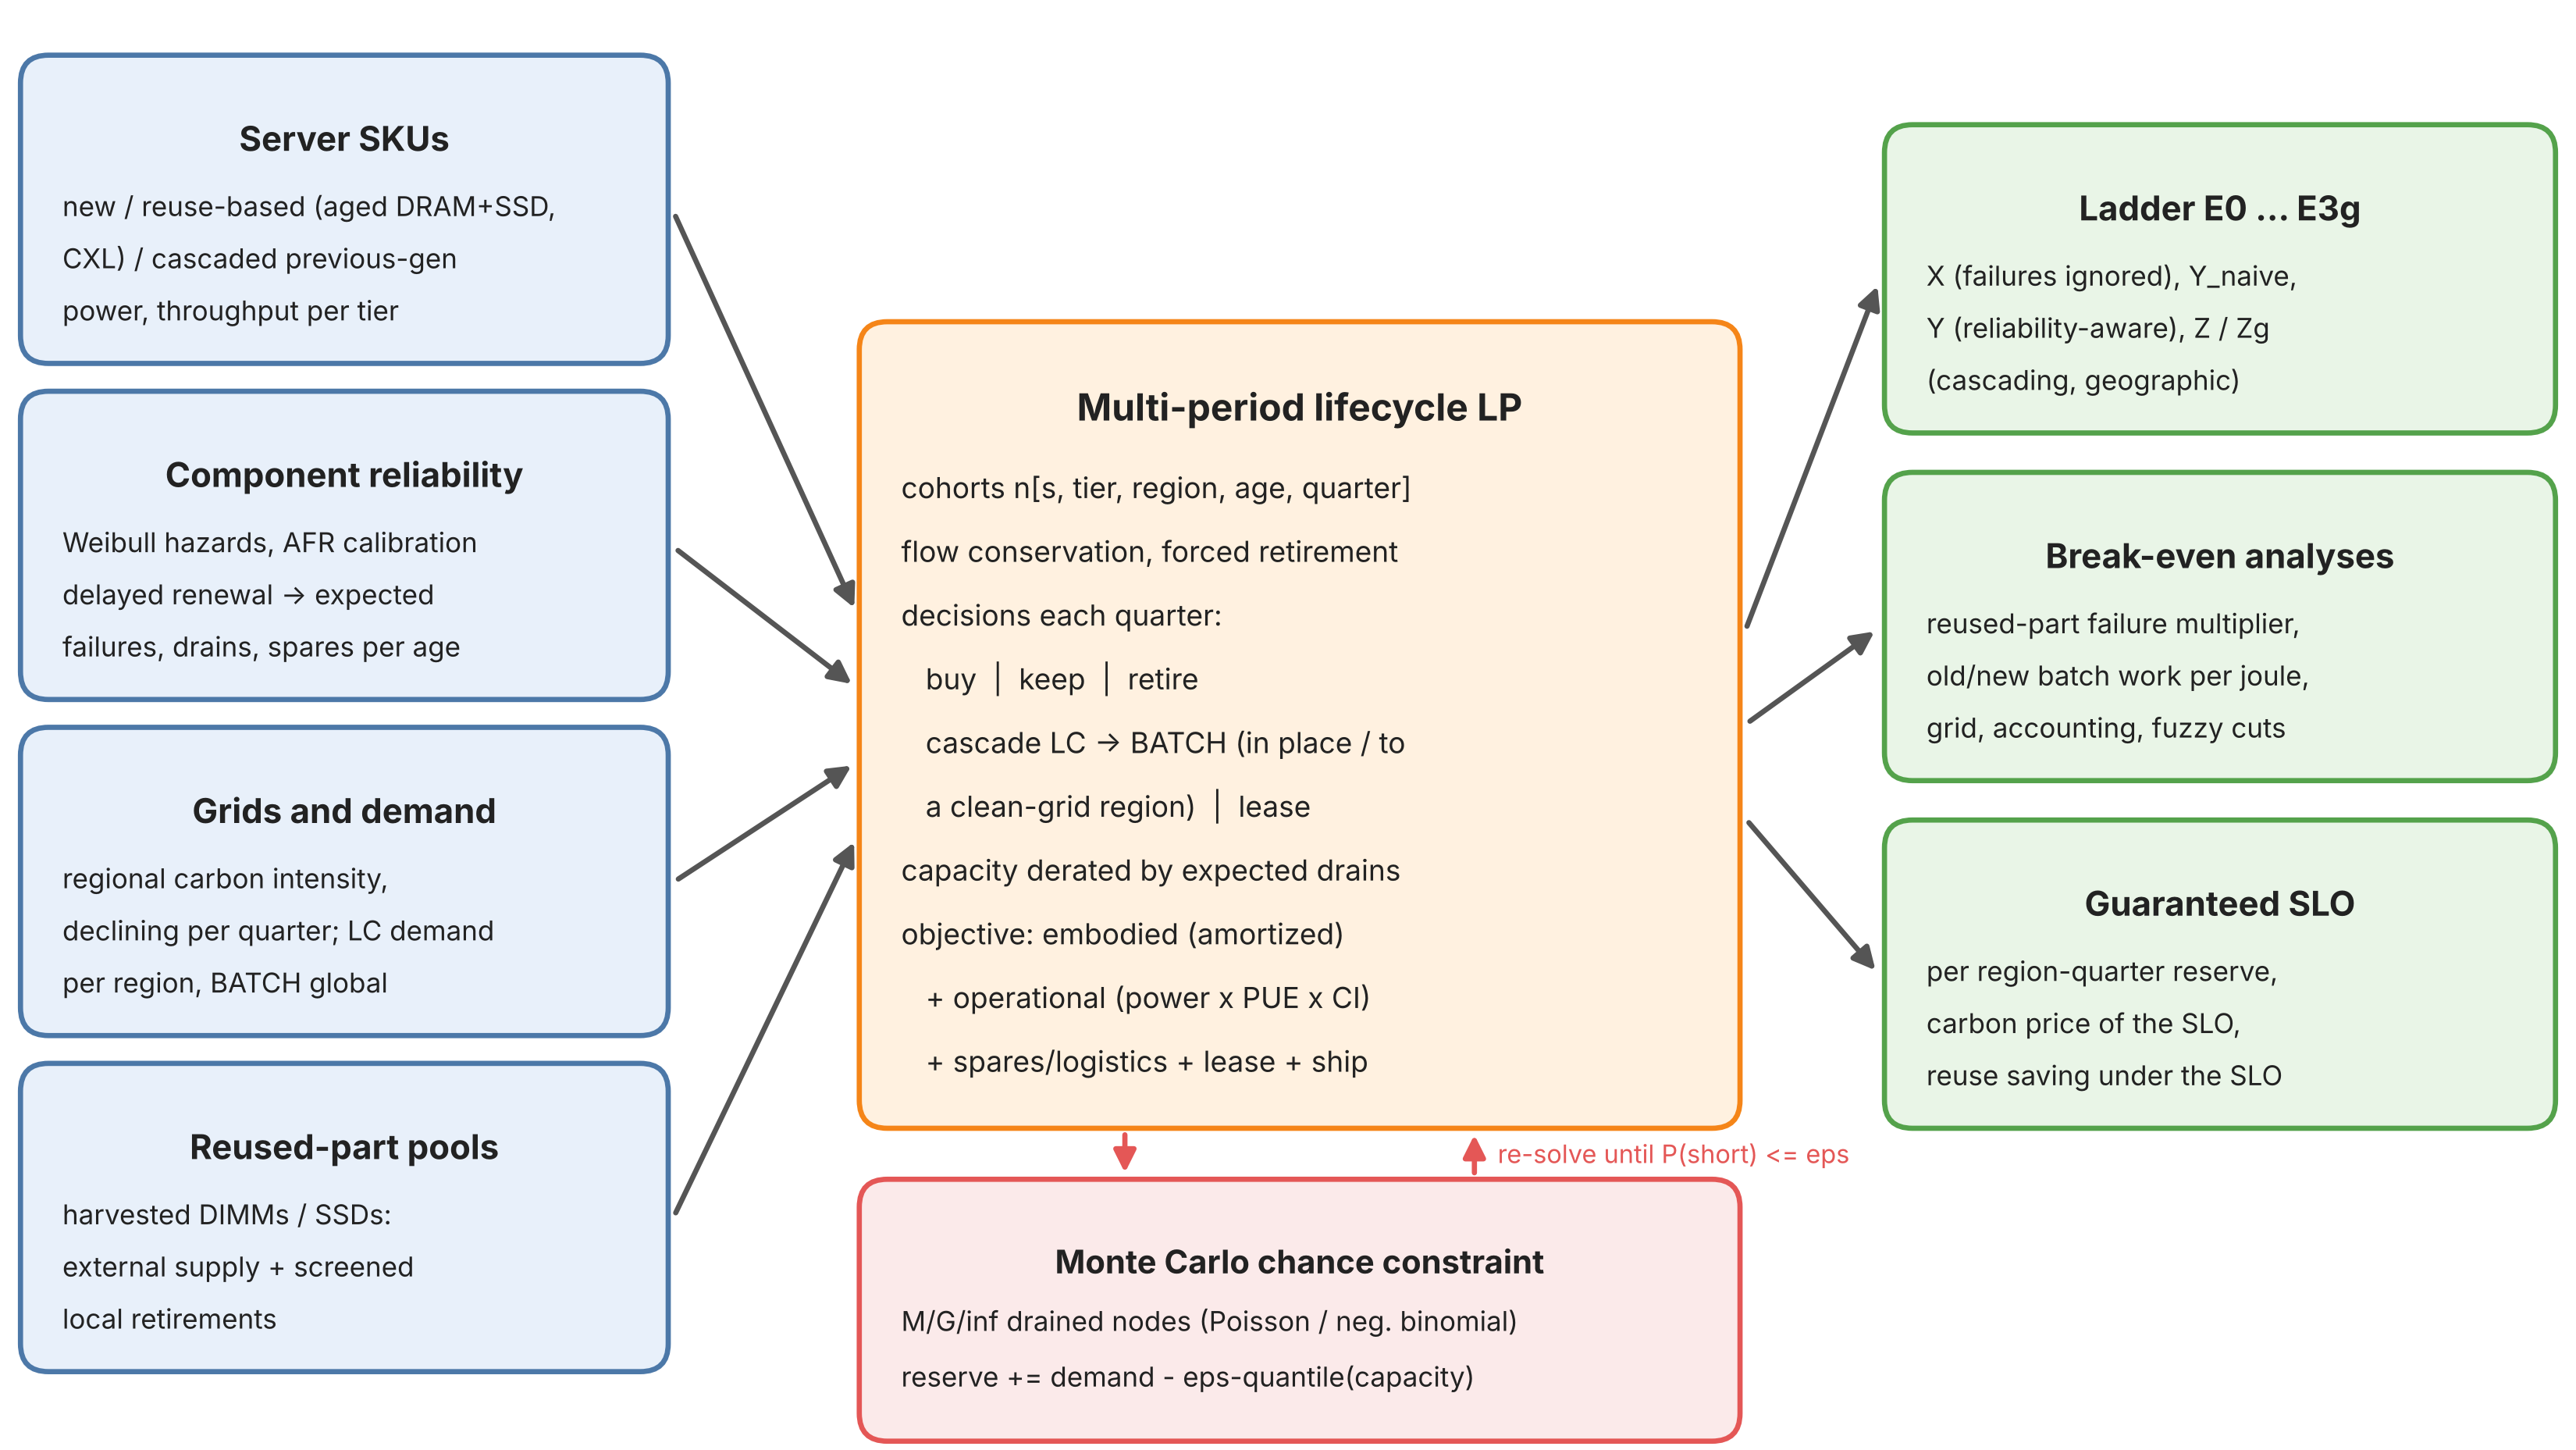
\includegraphics[width=\linewidth]{figures/fig_lifecycle_model_overview.png}
\end{center}
\caption{Overview of the reliability-aware lifecycle model. SKUs, component reliability (Weibull hazards, delayed renewal), regional grids and demand, and reused-part pools feed a multi-period LP over cohorts that each quarter decides to buy, keep, retire, cascade LC$\rightarrow$BATCH (in place or to a clean-grid region) or lease. An outer Monte Carlo loop models drained nodes as M/G/$\infty$ occupancy and adds reserve until $P(\text{short})\le\varepsilon$ in every region-quarter.}
\label{fig:overview}
\end{figure}

\subsection{Fleet State, Flow Conservation and Refurbishment}
\label{sec:method_state}
\label{sec:method_flow}
Time is discretized into quarters $t = 0,\dots,T-1$ with $T = 24$. Cohorts are indexed by SKU $s$, tier $\tau \in \{\text{LC}, \text{BATCH}\}$, region $r$ and node age $a$ (quarters within the current life); $n_{s\tau r a t} \ge 0$ counts nodes. Three SKUs are modelled. \texttt{new\_gpu} is a current-generation host with 8 GPUs, 2 standard CPUs, 32 DIMMs and 8 SSDs, all new. \texttt{green\_gpu} has the same 8 new GPUs and the same part counts, but 2 energy-efficient CPUs and 32 \emph{reused} DIMMs, attached over CXL~\citep{Sharma2024IntroductionCompute}, and 8 \emph{reused} SSDs, all entering at age $a_0=5$ years. It carries no extra memory: CXL enters the model only through a throughput multiplier (0.95 LC, 0.98 BATCH), power 50~W (idle) and 100~W (peak) below \texttt{new\_gpu}, and a platform embodied carbon of 1,600 rather than 1,500~kgCO$_2$e; failures are counted for the same 32 DIMMs and 8 SSDs at their reused age. \texttt{old\_gpu} is a previous-generation 8-GPU host cascaded as a whole (parts 4 years old). Node counts evolve as
\begin{equation}
\begin{split}
n_{s\tau r a t} = {} & n_{s\tau r,a-1,t-1} - x^{\text{ret}}_{s\tau r a t} + x^{\text{buy}}_{s\tau r t}\,[a=0] \\
& - [\tau=\text{LC}]\textstyle\sum_{r'} x^{\text{casc}}_{s r r' a t} + [\tau=\text{BATCH}]\textstyle\sum_{r''} x^{\text{casc}}_{s r'' r a t},
\end{split}
\label{eq:flow}
\end{equation}
with Iverson brackets $[\cdot]$, retirements $x^{\text{ret}}$, cascades $x^{\text{casc}}$ (from the LC tier of one region to the BATCH tier of another or the same region, keeping age; geographic cascades incur 300~kgCO$_2$e shipping) and purchases or builds $x^{\text{buy}}$, a fixed initial fleet and forced retirement at a maximum age. Refurbishment moves a node in an age window into a derived SKU at age 0 of a second life, replacing DIMMs (or DIMMs and SSDs) while carried parts keep their exact age and amortization schedule; one derived SKU exists per refurbishment age (Appendix~\ref{app:rel}).

\subsection{Age-Dependent Reliability as Precomputed Parameters}
\label{sec:method_rel}
Each component class $c \in \{\text{GPU}, \text{CPU}, \text{DIMM}, \text{SSD}\}$ has a Weibull hazard~\citep{Weibull1951StatisticalDistribution} over part age $a$ in years,
\begin{equation}
h_c(a) = \frac{k_c}{\eta_c}\left(\frac{a}{\eta_c}\right)^{k_c-1}, \qquad H_c(a) = \left(\frac{a}{\eta_c}\right)^{k_c},
\label{eq:weibull}
\end{equation}
with scale $\eta_c$ calibrated to the annualized failure rate (AFR). A reused part entering at age $a_0>0$ has first lifetime $F_{a_0}(x) = 1 - \exp(-[H_c(a_0+x) - H_c(a_0)])$, and failed parts are replaced by new spares, so each slot is a delayed renewal process with renewal function $M_{a_0}(x) = F_{a_0}(x) + \int_0^x M_0(x-y)\,dF_{a_0}(y)$, evaluated numerically. Expected failures $\lambda_{c,a}$, drained hours $d_{sa} = \sum_c N_{sc}\lambda_{c,a}\delta_c$ ($N_{sc}$ parts, drain time $\delta_c$), availability loss $\ell_{sa} = d_{sa}/H$ ($H$ hours per quarter), and spare and logistics carbon $q^{\text{spare}}_{sa}$, $q^{\text{log}}_{sa}$ per node-quarter enter the LP as coefficients. A proportional-hazards multiplier $m$ scales the hazard of reused parts beyond what their age predicts.

\emph{GPU hazard shape.} The GPU AFR comes from a published interruption report that gives a rate but no age profile, so the GPU hazard is constant (shape 1.0). Both \texttt{new\_gpu} and \texttt{green\_gpu} carry new GPUs of the same age, so they have identical GPU failures (4.36 per node over six years). GPU infant mortality or wear-out would therefore change both SKUs' drains and the overall headroom level, but not the GPU term of their difference. The age effect that separates them comes from the reused DIMMs (shape 1.6) and SSDs (shape 1.3), and previous-generation GPUs already have an increasing hazard (shape 1.3).

\subsection{Capacity, Reused-Part Pools and Objective}
\label{sec:method_cap}
\label{sec:method_obj}
Served work, in node-equivalents of a fully busy new host, satisfies
\begin{equation}
w_{s\tau r a t} \le n_{s\tau r a t}\,\theta_{s\tau}\, u \,\big(1 - \beta_\tau\, \ell_{s a}\big),
\label{eq:capacity}
\end{equation}
with relative throughput $\theta_{s\tau}$ (including the CXL multiplier), utilization cap $u$ and expected-value LC headroom multiplier $\beta_\tau$. LC demand $D_{rt}$ is regional. BATCH demand is global, which models delay-tolerant batch work that can be placed where capacity is~\citep{Wiesner2021LetsWait,Lechowicz2025LearningaugmentedCompetitive}. Network and data-locality costs of cross-region batch placement are not modelled beyond shipping carbon; this matters only where geographic cascading differs from in-place cascading, i.e., above energy parity (Section~\ref{sec:cascade}). Unserved demand is leased, with leased capacity carrying $\mu=1.3$ times the carbon of a new host per unit of work. Building a \texttt{green\_gpu} draws parts from harvest pools fed by pre-screened external supply plus a screening yield $\gamma$ times parts of hosts retired in the fleet (Eq.~\ref{eq:pool}). With all sums over $(s,\tau,r,a,t)$, the lifecycle-carbon objective is
\begin{equation}
\begin{split}
C = {} & \textstyle\sum \big[(e^{\text{emb}}_{s a} + q^{\text{spare}}_{sa} + q^{\text{log}}_{sa})\, n_{s\tau rat} + e^{\text{strand}}_{s a}\, x^{\text{ret}}_{s\tau rat}\big] \\
& + \textstyle\sum \text{PUE}\cdot\text{CI}_{r t}\,\big[P^{\text{idle}}_s (1-\ell_{sa}) H\, n_{s\tau rat} + \kappa_{s\tau}\, w_{s\tau rat}\big] + C^{\text{lease}} + C^{\text{ship}},
\end{split}
\label{eq:objective}
\end{equation}
where $e^{\text{emb}}$ is amortized embodied carbon, $e^{\text{strand}}$ the unamortized remainder charged on early retirement, $P^{\text{idle}}_s$ idle power, $\kappa_{s\tau}$ dynamic energy per unit of work and $\text{CI}_{rt}$ the regional, declining grid intensity. Reused parts carry zero embodied carbon by default (cut-off accounting). Cost is an alternative objective ($\varepsilon$-constraint front). At fleet scale we solve the LP relaxation (Section~\ref{sec:setup}).

\subsection{Experiment Ladder and Saving Metrics}
\label{sec:method_ladder}
\label{sec:method_uq}
E0 allows no reuse and is evaluated with failures ignored ($C^{\text{nf}}$) and counted ($C^{\text{f}}$). E1 allows reuse but ignores failures; E2a replays E1's plan with failures (drained capacity is covered by leasing); E2b plans reuse with reliability priced in; E3/E3g add in-place/geographic cascading; E0r, E4 and E5 add refurbishment. The savings, in percent, are
\begin{equation}
X = 1-\frac{C^{\text{nf}}_{\text{E1}}}{C^{\text{nf}}_{\text{E0}}}, \quad
Y_{\text{naive}} = 1-\frac{C^{\text{f}}_{\text{E2a}}}{C^{\text{f}}_{\text{E0}}}, \quad
Y = 1-\frac{C^{\text{f}}_{\text{E2b}}}{C^{\text{f}}_{\text{E0}}}, \quad
Z = \frac{C^{\text{f}}_{\text{E2b}} - C^{\text{f}}_{\text{E3}}}{C^{\text{f}}_{\text{E0}}},
\label{eq:savings}
\end{equation}
with $Z_g$ defined like $Z$ using E3g (both in pp). Because the no-reuse plan is feasible for E2b, $Y \ge 0$ by construction; the informative quantities are how fast $Y$ decays and where it reaches zero. Uncertainty is assessed by one-at-a-time (tornado) sensitivity, triangular fuzzy factors on failure rates ($\times[0.5,1,3]$), embodied carbon ($\times[0.5,1,2]$) and the CXL multiplier ($[0.85,0.95,1.0]$) propagated to $Y$ by $\alpha$-cuts, and sweeps.

\subsection{Chance-Constrained SLO Headroom}
\label{sec:method_cc}
\emph{Shortfall semantics.} Demand $D_{rt}$ is constant within a quarter. $P(\text{short}_{rt})$ is the probability that, at a uniformly random instant of quarter $t$, the LC capacity of region $r$ net of drained nodes, $\text{capacity}_{rt}$, is below $D_{rt}$. With stationary drain occupancy within the quarter this equals the expected fraction of the quarter spent in shortfall; it is not a worst-case-within-quarter measure. \emph{Occupancy model.} Failures of the many component slots of a region's LC cohorts form approximately a Poisson stream, and each failure drains its node for a drain time, so the number of drained nodes is M/G/$\infty$ occupancy~\citep{Eick1993PhysicsMtg}, Poisson with mean $\mu_{rt} = \sum_i N_i d_i / H$ over LC cohorts $i$. Correlated failures (e.g., a common firmware or batch defect within a region) are represented by a common random factor on the failure rate: a Gamma-distributed factor with mean 1 and variance $1/k$ turns the Poisson occupancy into a negative binomial with mean $\mu_{rt}$ and variance $\mu_{rt} + \mu_{rt}^2/k$ (smaller $k$, stronger correlation). We use $k=2$ and $k=0.5$ as illustrative levels, not fitted values. A per-region-quarter reserve $R_{rt}$ enters through
\begin{equation}
\textstyle\sum_{s,a} n_{s,\text{LC},r a t}\,\theta_{s,\text{LC}}\,u + L_{rt} \ge D_{rt} + R_{rt},
\label{eq:reserve}
\end{equation}
with leased LC capacity $L_{rt}$, and we require $P(\text{capacity}_{rt} < D_{rt}) \le \varepsilon$ in every region-quarter. Algorithm~\ref{alg:cc} (Appendix~\ref{app:results}) solves the plan, samples capacity per region-quarter, adds the gap between demand and the $\varepsilon$-quantile of capacity to $R_{rt}$, and re-solves until all gaps are within 0.05\% of demand; reserves only grow. The loop is a feasibility heuristic without an optimality guarantee: its final plan is validated by an independent replay with 50,000 samples, so its carbon is an upper bound, up to sampling error and tolerance, on the cheapest plan meeting the constraint in this model. Because the constraints are per-region-quarter marginals, correlation \emph{across} regions or quarters does not change them; it would matter for a joint guarantee (e.g., no region short at once), which we do not impose. The \emph{SLO carbon price} is the relative carbon increase of the chance-constrained plan over its expected-value plan.
%%%%%%%%% METHOD %%%%%%%%%

\section{Experiments}
\label{sec:experiments}
%%%%%%%%% EXPERIMENTS %%%%%%%%%
\subsection{Experimental Setup}
\label{sec:setup}
\paragraph{Scenarios and parameters.} \emph{Node-level study:} one 8-GPU node per SKU over six years at 60\% utilization on a clean, mixed and dirty grid (base-year 40, 250 and 650~gCO$_2$e/kWh, declining 2, 5 and 3\%/yr; PUE 1.2). \emph{Pilot fleet:} 3 years, one region, 24 previous- and 12 current-generation hosts. \emph{Reference fleet:} 24 quarters, three regions, about 1,750 initial hosts, LC demand growing 25--30\% and global BATCH demand 35\% per year, and reused-part pools fed by 2,400 DIMMs and 600 SSDs per quarter. Full scenario, SKU, component and cost parameters are in Appendix~\ref{app:params}. The GPU AFR of 0.0868 is derived from a published interruption report; all other parameters are engineering assumptions with swept ranges. \textbf{GPU throughput, power and the CXL slowdown are placeholders: the prepared GPU measurements (Appendix~\ref{app:measure}) have not been executed, and no measured GPU results are reported.}

\paragraph{Baselines and implementation.} Baselines are the no-reuse fleet (E0), the failure-blind reuse plan (E1/E2a), and expected-value headroom. \emph{Headroom convention:} all results use $\beta_{\text{LC}}=3$ and $u=0.8$ except the chance-constrained study (Section~\ref{sec:slo}), whose expected-value baseline uses $\beta_{\text{LC}}=1$ because the reserve replaces the derating. At $m=1$ the two baselines give the same $Y$ (0.775\% at $\beta=1$ and at $\beta=3$, Table~\ref{tab:headroom_app}); at $m=3$ they give 0.480\% and 0.475\%. The model is solved with HiGHS through a Python layer. On the pilot, the mixed-integer model hit a 300~s limit without proving optimality, while the LP relaxation solved in under 1~s, matched the integer $X$ and $Y$ within about 0.05~pp and gave identical $X$, $Y$, $Z$ at 1$\times$ and 50$\times$ fleet scale. We therefore use the LP at fleet scale, where cohorts contain many nodes, but treat effects below about 0.05~pp as unresolved. A full E0--E3g ladder on the reference fleet solves in about 4~s.

\subsection{Node-Level Lifecycle Carbon and Grid Dependence}
\label{sec:node}
For \texttt{new\_gpu} on the mixed grid (LC, failures counted), operational carbon is about 91\% of the six-year total (Table~\ref{tab:node}). Reusing DRAM and SSDs cuts embodied carbon by about two thirds (8.3 to 2.9~tCO$_2$e per node) but total carbon by only about 6\%. The per-unit-of-work saving is therefore strongly grid-dependent (Table~\ref{tab:node_saving}): about 16\% (LC) and 19\% (BATCH) on the clean grid, 0.9\% and 4.0\% on the mixed grid, and $-2.2\%$ and 1.0\% on the dirty grid, where the 5\% LC throughput loss of the CXL multiplier costs more operational carbon than reuse saves. Counting failures, spares, logistics and drains erodes the node-level saving by only 0.1--2.2~pp: aged DIMMs nearly double DIMM failures (9.67 versus 5.43 per node), but GPU failures, common to both SKUs, dominate drained hours (394 versus 359~h).

\paragraph{The reuse SKU bundles SSD reuse and DRAM-over-CXL reuse.} In the model the CXL slowdown is caused entirely by the reused DRAM, while reused SSDs carry no throughput penalty. A back-of-envelope decomposition of logged parameters (a derivation, not a model run) suggests that the two pull in opposite directions on the mixed grid. Of the 5,452~kgCO$_2$e embodied reduction per node ($8{,}312-2{,}860$), reused SSDs contribute $8\times 614 = 4{,}912$ (88\% of the gross 5,552) and reused DIMMs $32\times 20=640$, less the +100~kgCO$_2$e platform delta that includes the CXL controller, i.e., about 540 net. The 5\% LC slowdown instead raises operational carbon per unit of work by about $95{,}511\times(1/0.95-1)\approx 5.0$~tCO$_2$e per node, roughly nine times the net DRAM credit; consistently, the tornado gives a saving of 5.88\% at a CXL multiplier of 1.0 versus 0.93\% at 0.95 (Table~\ref{tab:tornado_app}). On these numbers DRAM-over-CXL reuse would pay only where the node's operational carbon is below about $540/(1/0.95-1)\approx 10$~tCO$_2$e, roughly a tenth of the mixed-grid value, and a SKU with reused SSDs and new local DRAM might save roughly 5\% (5.88\% minus about 0.5~pp of forgone net DIMM credit) rather than 0.93\%. We did not run such a SKU. The estimate ignores that new DIMMs fail less (5.43 versus 9.67 failures) and assumes the power deltas belong to the CPUs; the SSD credit itself depends on the assumed 614~kgCO$_2$e per SSD (the saving is $-2.49\%$ at 150). We therefore state it as a hypothesis for future work, and our node and fleet results apply to the bundle, not to either intervention alone.

\subsection{What the Conclusions Depend On: Break-Even Map}
\label{sec:breakeven}
Table~\ref{tab:breakeven} collects, for each qualitative conclusion, the parameter that controls it and the value at which it flips; the subsections below give the evidence. The CXL multiplier dominates the node-level tornado (Figure~\ref{fig:tornado}): over 0.85--1.0 the mixed-grid LC saving moves from $-10.7\%$ to 5.9\%, about three times the swing of the next parameter. By linear interpolation of the tornado end points, the mixed-grid saving is positive only if the CXL slowdown is below about 6\% (multiplier $\geq 0.94$), the grid intensity is below about 320~gCO$_2$e/kWh, and the reuse host's peak power does not exceed the new host's by more than about 15~W. The CXL multiplier acts only on \texttt{green\_gpu} and the old/new energy ratio only on \texttt{old\_gpu}, so the sign of the node-level saving and the value of cascading are governed by different parameters; we have not computed their joint map.

\begin{table}[t]
\caption{Break-even map: the parameter that controls each conclusion, its baseline value, and the value at which the conclusion flips. Values marked $^\ast$ are linear interpolations or readings between swept points, $^\dagger$ first-order derivations holding the replayed plan fixed (Section~\ref{sec:fleet}), $^\S$ a back-of-envelope derivation, not a model run (Section~\ref{sec:node}); $^\ddagger$ a bracket between swept points ($Y=0.209\%$ at $m=5$, $0$ at $m=8$; no runs in between), so 8 is an upper bound. Placeholder parameters are marked (P). The failure-blind rows mainly measure the cost of ignoring drains ($Y_{\text{naive}}=-0.557\%$ even when reuse saves nothing; Section~\ref{sec:fleet}).}
\label{tab:breakeven}
\centering
\small
\resizebox{\linewidth}{!}{%
\begin{tabular}{lllr}
\toprule
Conclusion & Controlling parameter & Baseline & Flips at \\
\midrule
Mixed-grid LC node saving $>0$ & CXL LC throughput multiplier (P) & 0.95 & $\approx 0.94^\ast$ \\
 & mixed-grid intensity (gCO$_2$e/kWh) & 250 & $\approx 320^\ast$ \\
 & reuse-host peak-power delta (W) & $-100$ & $\approx +15^\ast$ \\
DRAM-over-CXL reuse alone pays & node operational carbon (t) & $\approx 95$ & $\approx 10^\S$ \\
Failure-blind fleet saving $Y_{\text{naive}}>0$ & reused-part failure multiplier $m$ & 1 & $\approx 2.1^\ast$ \\
 & leased-capacity carbon multiplier $\mu$ & 1.3 & $\approx 1.39^\dagger$ \\
Reliability-aware plan still reuses ($Y>0$) & reused-part failure multiplier $m$ & 1 & in $(5, 8]^\ddagger$ \\
Cascading pays & old/new BATCH work per joule (P) & 0.70 & $\approx 0.93$--$1.0^\ast$ \\
Refurbishment is chosen & new-DIMM AFR and $m$ & 0.01, 1 & AFR $\ge 0.03$, $m\in\{3,5\}$ \\
\bottomrule
\end{tabular}%
}
\end{table}

\subsection{Fleet-Level Savings: Failure-Blind vs.\ Reliability-Aware Planning}
\label{sec:fleet}
Table~\ref{tab:fleet_savings} reports fleet savings. On the reference fleet $X \approx 0.85\%$, $Y_{\text{naive}} \approx 0.20\%$ and $Y \approx 0.78\%$. These savings are small because operational energy is about 94\% and embodied carbon only about 5\% of the no-reuse fleet's lifecycle carbon (Table~\ref{tab:ladder}), and existing hosts are unaffected by reuse. This share rests on assumed embodied values, including 150~kgCO$_2$e per GPU (1.2 of a new host's 8.3~tCO$_2$e; Table~\ref{tab:params}); the fuzzy analysis below doubles all embodied carbon at most, and larger factors were not run. They are of the same order as their uncertainty: fuzzy $\alpha$-cuts give $Y\in[0, 2.64]\%$ at $\alpha=0$ and $[0.27, 1.49]\%$ at $\alpha=0.5$, and across six embodied-carbon conventions $Y$ ranges from 0 (reused parts charged as new) to 1.42\% (Table~\ref{tab:accounting}). For a fleet of this composition, then, component reuse is not a material carbon lever: the saving is not distinguishable from zero under joint uncertainty, and it disappears entirely when reused parts are charged as new. The ordering is more robust than the level: $Y > Y_{\text{naive}}$ in every fleet, grid, accounting convention and multiplier setting we ran, and the grid dependence carries over (clean-only $Y \approx 5.0\%$, dirty-only $\approx 0.09\%$).

\begin{table}[t]
\caption{Fleet savings relative to the no-reuse fleet (\%; $Z$ in pp), LP relaxation.}
\label{tab:fleet_savings}
\centering
\small
\begin{tabular}{llrrrr}
\toprule
Scenario & Fleet & $X$ & $Y_{\text{naive}}$ & $Y$ & $Z$ (pp) \\
\midrule
Pilot & clean / mixed / dirty & 8.65 / 0.97 / 0.18 & 7.07 / 0.33 / $-0.33$ & 7.49 / 0.85 / 0.15 & 0.00 \\
\midrule
Reference & three-grid fleet & 0.848 & 0.195 & 0.775 & 0.005 \\
Reference & clean grid only & 5.766 & 4.584 & 5.028 & 0.005 \\
Reference & mixed grid only & 0.675 & 0.039 & 0.568 & 0.000 \\
Reference & dirty grid only & 0.103 & $-0.443$ & 0.087 & 0.000 \\
\bottomrule
\end{tabular}
\end{table}

\paragraph{Why failure-blind planning loses, and what its break-evens measure.} The failure-blind plan (E1 replayed as E2a) is a naive reference, not a strong operator baseline: it installs no headroom for drains. The realistic baseline, an operator who derates capacity by the expected drain and prices spares, is what E2b adds over E1, and it already recovers most of the saving: $Y/X \approx 0.775/0.848 \approx 0.91$. Figure~\ref{fig:ladder} (Appendix~\ref{app:figures}; values in Table~\ref{tab:ladder}) shows the mechanism: the replay of the failure-blind plan must lease 13,104~tCO$_2$e of capacity versus 530~tCO$_2$e for the reliability-aware plan, partly offset by 8.8~ktCO$_2$e less operational and 0.8~ktCO$_2$e less embodied carbon. Most of this loss is the cost of ignoring drains, not of reuse. When reused parts are charged as new, reuse yields no failure-free saving ($X=0$), yet $Y_{\text{naive}}=-0.557\%$ (Table~\ref{tab:accounting}); a failure-blind plan thus loses about half a percent even without any benefit from reuse. The failure-blind break-evens ($m\approx 2.1$; $\mu\approx 1.39$, below) therefore mark where reuse's saving no longer covers the cost of ignoring drains, and largely measure that cost. A separate failure-blind no-reuse replay was not run, so we cannot restate them against it; as an indicative difference only (the accounting conventions differ), $0.195-(-0.557)\approx 0.75$~pp is close to $Y=0.775\%$. The loss also depends on the leased-capacity carbon multiplier $\mu=1.3$, which we did not sweep. Because E2a is a fixed plan replayed, its leased carbon is proportional to $\mu$: to first order, each 0.1 change in $\mu$ moves $Y_{\text{naive}}$ by about 0.21~pp, so $Y_{\text{naive}}$ would be about 0.81\% at $\mu=1.0$ and reaches zero at $\mu\approx 1.39$, whereas the fixed E2b plan moves by only about 0.008~pp per 0.1 of $\mu$ (Appendix~\ref{app:results}). Once derating is applied, its amount hardly matters: $Y$ stays within 0.775--0.806\% for headroom multipliers 1--10 and utilization caps 0.5--0.8 (Table~\ref{tab:headroom_app}). The practical lesson is only that some derating for drains is needed, which operators already apply.

\paragraph{Break-even reliability of reused parts.} Figure~\ref{fig:breakeven} (Appendix~\ref{app:figures}; Table~\ref{tab:mult_app}) shows how fast each planner's saving decays. The failure-blind saving crosses zero at $m\approx 2.1$ (interpolated between $m=2$ and 3) and reaches about $-2.3\%$ at $m=20$. The reliability-aware planner progressively buys fewer reuse-based hosts, so $Y$ declines gradually (about 0.62\% at $m=2$, 0.48\% at $m=3$, 0.21\% at $m=5$) and is 0 at the next swept point, $m=8$. The crossover therefore lies between 5 and 8; 8 is an upper bound, not an estimate. Linear extrapolation of the $m=3$ and $m=5$ points would place it near $m\approx 6.6$, but no runs between 5 and 8 exist. That $Y\ge 0$ is a property of optimization, since no reuse is always feasible; the informative result is that reuse remains worthwhile up to at least a fivefold excess failure rate of reused parts. $Y$ is only weakly sensitive to the reused-part entry age: 0.795\%, 0.775\% and 0.759\% for entry ages of 3, 5 and 7 years (Table~\ref{tab:entry_app}).

\subsection{When Does Cascading Pay?}
\label{sec:cascade}
At the placeholder old-GPU BATCH throughput of 0.45 (old/new BATCH work per joule 0.70), cascading adds essentially nothing: $Z = Z_g = 0.005$~pp, below the model's resolution. Figure~\ref{fig:cascade} (Appendix~\ref{app:figures}; values in Table~\ref{tab:cascade_app}) shows that the benefit stays near zero below parity (0.03~pp at 0.93), begins near parity, and grows roughly linearly above it to $Z \approx 0.35$~pp and $Z_g \approx 0.52$~pp at 1.87. Above parity, geographic cascading to the clean-grid BATCH tier adds roughly 50--70\% on top of in-place cascading. Cascading only avoids the embodied carbon of new hosts, which is small relative to a GPU host's operational carbon. Whether real previous-generation GPUs lie above or below parity is what the pending per-generation tokens-per-joule measurements must decide.

\subsection{Guaranteeing LC SLOs Under Correlated Failures}
\label{sec:slo}
\paragraph{Expected-value headroom is not enough.} Replaying the expected-value plans ($\beta_{\text{LC}}=3$) over the 72 region-quarters (Table~\ref{tab:ev_risk}) gives low mean shortfall probability (0.2--2.6\%), but the worst region-quarter of the reuse plan reaches about 14.5\% with independent and 15.5\% with correlated failures. Correlated failures raise the number of region-quarters above 1\% from 5 to 48 (no reuse) and from 4 to 44 (reuse). With independent failures the reuse plan's mean (0.40\% versus 0.20\%) and its count of region-quarters above 1\% (4 versus 5) are close to the no-reuse plan's, so its higher worst case (14.5\% versus 2.7\%) is concentrated in very few region-quarters; the per-region-quarter breakdown that would identify them was not logged.

\paragraph{Chance-constrained plans.} Figure~\ref{fig:slo} and Tables~\ref{tab:cc} and~\ref{tab:cc_app} report results for $m=1$ and $m=3$. \emph{Baseline:} unlike Table~\ref{tab:ev_risk} and all other results, which use $\beta_{\text{LC}}=3$, the expected-value baseline of this study uses $\beta_{\text{LC}}=1$, because the chance-constrained reserve replaces the derating rather than adding to it. The SLO carbon price is therefore measured against the $\beta_{\text{LC}}=1$ plan, not against the $\beta_{\text{LC}}=3$ plan whose exposure is shown above; the two give the same $Y$ at $m=1$ (0.775\%) and nearly the same at $m=3$ (0.480\% versus 0.475\%), but their carbon difference was not logged, so a price relative to the $\beta_{\text{LC}}=3$ plan cannot be reported. The loop converged in 4 to 15 iterations. At the 0.1\% target, $k=0.5$ needs about 2.5 times the reserve of independent failures (Table~\ref{tab:reserve_app}), and the SLO carbon price roughly doubles to triples from independent to strongly correlated failures (0.30\% to 0.79\% for the reuse plan). In every setting the reuse plan pays a slightly lower SLO carbon price than the no-reuse plan, so the reuse saving under a guaranteed SLO changes by $+0.01$ to $+0.04$~pp at $m=1$ and by $+0.004$ to $+0.02$~pp at $m=3$. All of these changes are below the model's 0.05~pp resolution, and across three Monte Carlo seeds the saving at 0.1\%, $k=0.5$ ranges from 0.800\% to 0.814\% (Table~\ref{tab:seeds_app}). This is a null result, and we report it as one: \emph{no detectable carbon penalty} for reuse under an SLO guarantee, not an increase in the saving. Its practical content is that the concern motivating the study, that less reliable reused parts would make SLO headroom costlier, is not borne out at this resolution.

\begin{figure}[t]
\begin{center}
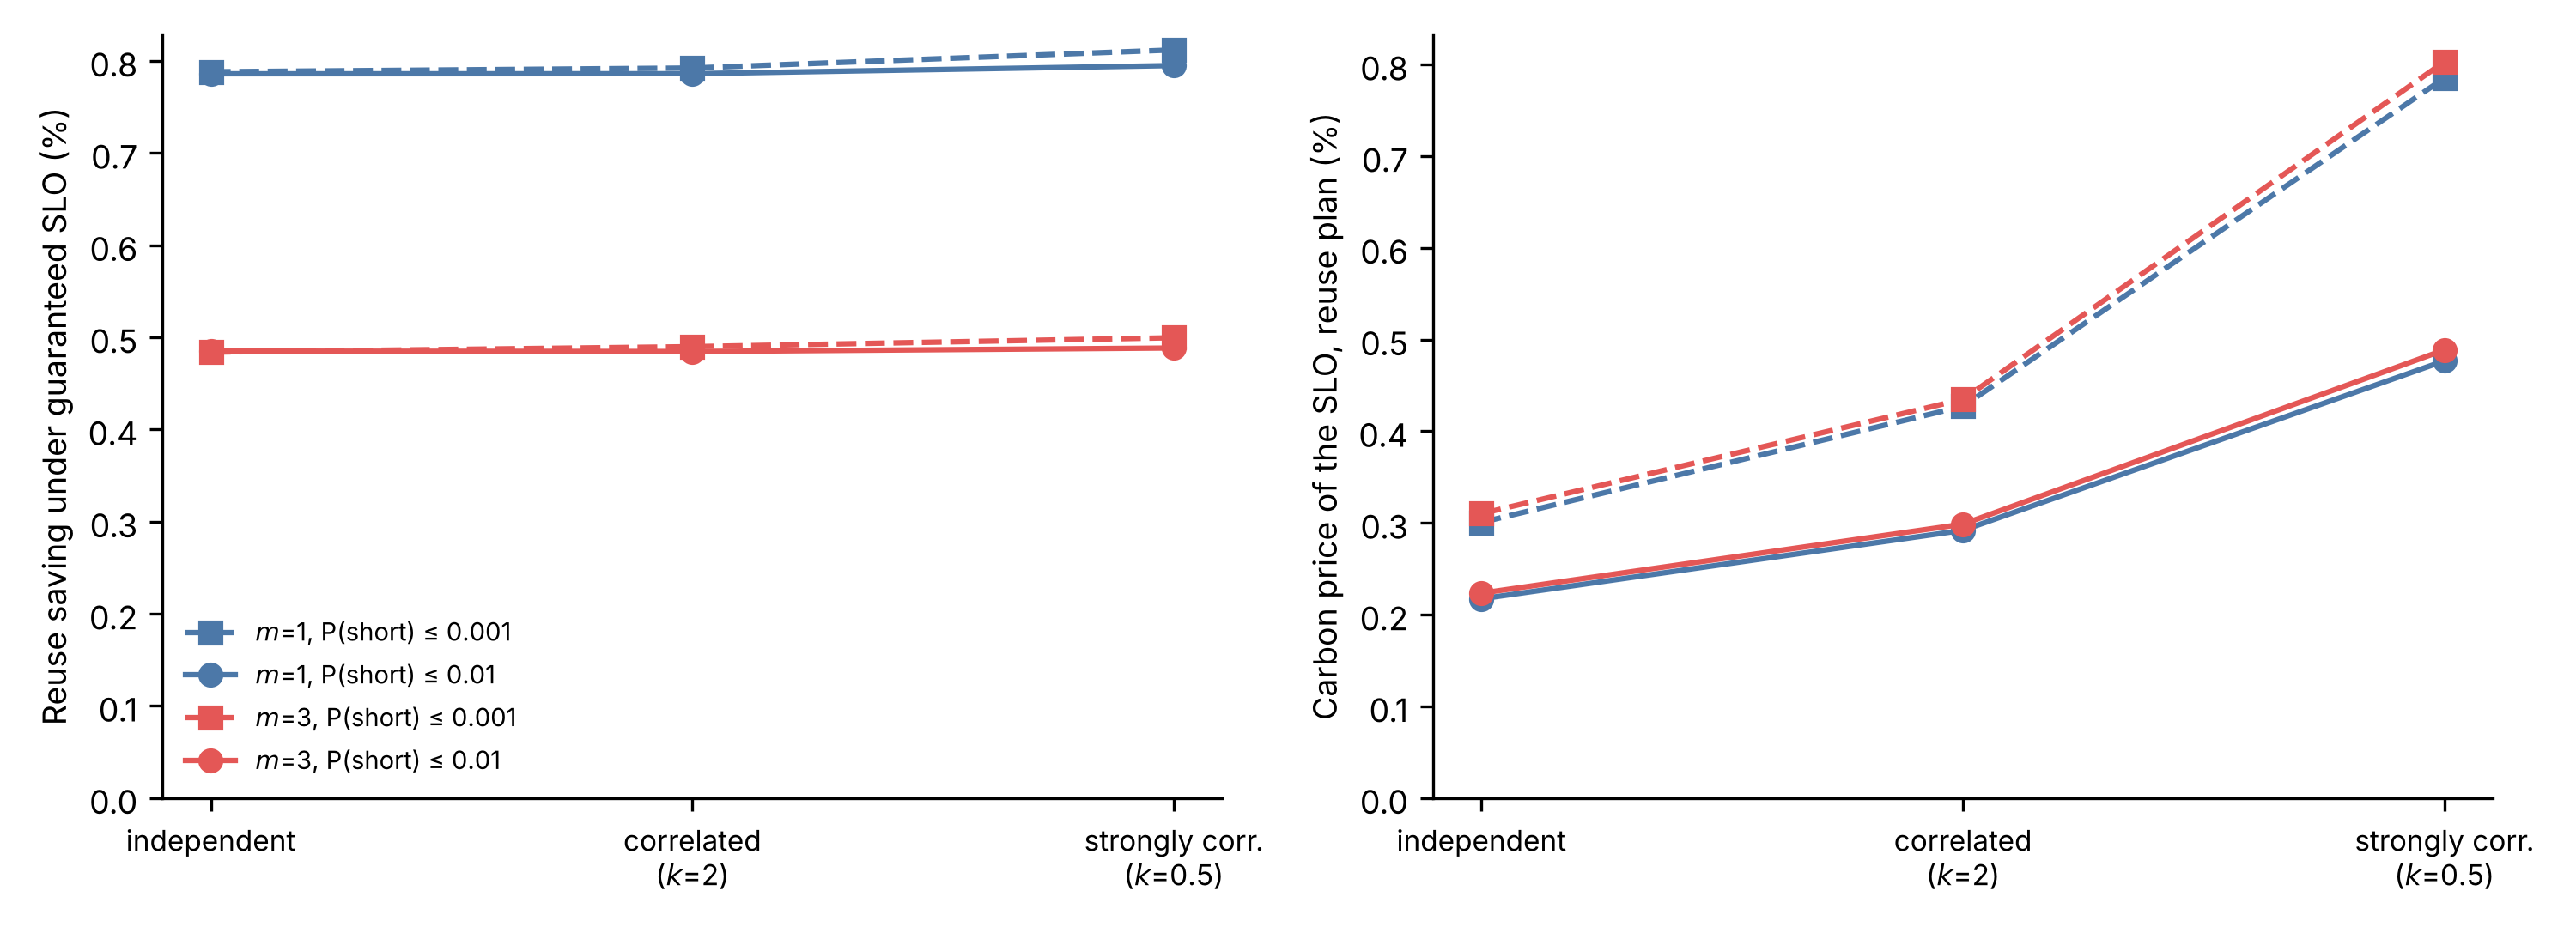
\includegraphics[width=\linewidth]{figures/fig_chance_constrained_slo.png}
\end{center}
\caption{Left: reuse saving under a guaranteed LC SLO (per-region-quarter shortfall probability at most 1\% or 0.1\%) for independent, correlated ($k=2$) and strongly correlated ($k=0.5$) failures, with $m=1$ or $m=3$. Right: SLO carbon price of the reuse plan relative to its expected-value plan. Differences in the left panel are below the model's 0.05~pp resolution, i.e., no detectable carbon penalty.}
\label{fig:slo}
\end{figure}

\paragraph{What drives the lower price.} At 0.1\%, $k=0.5$, $m=1$ (Table~\ref{tab:composition}), the reserve's added carbon is mostly operational energy (83\% without and 85\% with reuse; embodied 14\% and 12\%). The log does not split this operational share into idle and dynamic energy; reserve capacity is idle by design, so we expect most of it to be idle energy, but that is not measured. The reuse plan places 21.7\% of its added capacity on reuse-based hosts and its reserve carries 214~tCO$_2$e (5.3\%) less added carbon: about 110~tCO$_2$e less embodied and 115~tCO$_2$e less operational carbon, partly offset by about 8~tCO$_2$e \emph{more} spares and logistics (its reused parts fail more), with the remaining few tCO$_2$e due to rounding of the logged components (Appendix~\ref{app:reconcile}). Across three seeds it needs 2.6--3.6\% less added capacity. The $m=3$ runs act as a partial control: there the reuse plan needs slightly \emph{more} reserve than the no-reuse plan in most settings (e.g., 527.7 versus 516.3 node-equivalent-quarters at 0.1\%, independent), yet still pays a lower price. This points to the lower carbon per unit of reserve on reuse-based hosts, rather than a smaller reserve, as the primary cause, although we have not isolated it further. Validated worst-case probabilities are 0.96--1.07\% at the 1\% target and 0.10--0.13\% at 0.1\%. The largest, 0.13\% (no-reuse plan, independent failures), exceeds its target by about two standard errors (about 0.014~pp at 0.1\% with 50,000 samples); as the maximum over 72 noisy region-quarter estimates, and with the loop stopping at gaps within 0.05\% of demand, such an excess is plausible, but it is an exceedance, not agreement within one standard error. A slightly conservative stopping rule would be expected to remove it; it was not run.

\subsection{Refurbishment and Carbon-Cost Trade-off}
\label{sec:refurb}
\label{sec:robustness}
With baseline parameters the planner never refurbishes (E2b and E4 both 0.775\%; E5 with all levers 0.780\%): new DIMMs' embodied carbon and the 24~h downtime outweigh the failures avoided. Refurbishment is chosen only for reuse-based hosts whose recycled DIMMs fail heavily, for at most 0.015~pp extra saving (Table~\ref{tab:refurb}). Building it exactly required one derived SKU per refurbishment age. Approximate treatments over-credit refurbishment (Appendix~\ref{app:rel}); one, counting harvested parts every quarter instead of once, apparently doubled the clean-grid saving, which is a practical caution for lifecycle models. On the carbon-cost $\varepsilon$-constraint front (Figure~\ref{fig:pareto}, whose axis values are in ktCO$_2$e; Table~\ref{tab:pareto_app}), the cost-minimal plan emits 2.6\% more carbon than the carbon-minimal plan while costing about 14\% less. Here the carbon-minimal plan is point 7 (486.8~ktCO$_2$e, USD 1.680 billion): the logged endpoint has the same printed carbon at higher cost (USD 1.719 billion), so it is dominated at printed precision; whether it was solved lexicographically is not recorded. About two thirds of the carbon gain is available at 2.8\% and over 80\% at 5.6\% extra cost.
%%%%%%%%% EXPERIMENTS %%%%%%%%%

\section{Conclusion}
\label{sec:conclusion}
%%%%%%%%% CONCLUSION %%%%%%%%%
We presented a reliability-aware, multi-period lifecycle-carbon LP for LLM-inference fleets with a chance-constrained LC headroom loop. Its answer to the title question is conditional, and the model makes the conditions explicit (Table~\ref{tab:breakeven}). Reuse pays clearly per unit of work on clean grids. On mixed grids it pays only if the CXL slowdown stays below about 6\%. At fleet scale, where operational energy dominates, the saving is below 1\% and not distinguishable from zero under joint uncertainty, a negative result for reuse as a fleet-level carbon lever. Simple derating for expected drains retains about 90\% of the failure-free saving and keeps reuse worthwhile up to at least a fivefold excess failure rate of reused parts (the crossover lies between 5 and 8), whereas a naive failure-blind plan loses most of it, mainly because ignoring drains costs carbon even without reuse. Most of the reuse SKU's embodied saving comes from reused SSDs and its slowdown from reused DRAM over CXL; a SKU with reused SSDs and new local DRAM is the natural next experiment. Cascading needs old/new energy parity. Expected-value headroom leaves individual region-quarters exposed, and guaranteeing an LC SLO shows no detectable carbon penalty for reuse.

\paragraph{Limitations.} All results are model outputs. GPU throughput, power and the CXL slowdown are placeholders pending measurements that have been prepared but not run (Appendix~\ref{app:measure}), so the sign of the mixed-grid saving and the value of cascading are open until those measurements exist. Other parameters except the GPU AFR are engineering assumptions; the negative-binomial dispersions are illustrative; correlation across regions and quarters, network and data-locality constraints on batch placement, demand uncertainty, supply limits on leased capacity, and integrality effects below 0.05~pp are not modelled; and we make no claims about training fleets. Modelling choices cut both ways: cut-off accounting favours reuse ($Y=0$ when reused parts are charged as new), whereas a possible memory-capacity benefit of CXL (e.g., a larger KV cache) is not credited and CXL controller embodied carbon is folded into the +100~kgCO$_2$e platform delta. All GPU-related interruptions in the source report are treated as failures with a 72~h drain; if a share were transient, GPU drains would fall equally for \texttt{new\_gpu} and \texttt{green\_gpu}, lowering the headroom level of both. The reuse SKU bundles SSD and DRAM-over-CXL reuse, and the decomposition separating them is a derivation, not a model run. Cited numbers should be quoted together with these caveats to avoid overstating carbon savings.

\section*{Reproducibility Statement}
The model is a cohort-by-age LP (Section~\ref{sec:method}) solved with HiGHS through a Python modeling layer; all parameters, scenarios and sweep ranges are listed in Section~\ref{sec:setup} and Appendices~\ref{app:params}--\ref{app:results}. A suite of 48 tests, including a hand-calculated single-SKU case, conservation of embodied carbon at every refurbishment age and reused-part pool balance, accompanies the model. Chance-constrained plans are validated by independent Monte Carlo replay with 50,000 samples per region-quarter; the seed study uses seeds 0, 101 and 202.
%%%%%%%%% CONCLUSION %%%%%%%%%

%%%%%%%%% REFERENCES %%%%%%%%%
\bibliography{references}
\bibliographystyle{iclr2025_conference}
%%%%%%%%% REFERENCES %%%%%%%%%

%%%%%%%%% Appendix %%%%%%%%%
\clearpage
\appendix

\section{Full Parameter Tables and Provenance}
\label{app:params}
Table~\ref{tab:params} lists SKU and component parameters. Table~\ref{tab:costs} lists cost and logistics parameters used for the carbon-cost front; electricity is priced at the meter times PUE. Sensitivity ranges for the ten most influential parameters are given in Table~\ref{tab:tornado_app}.

\begin{table}[h]
\caption{Cost and logistics parameters (engineering assumptions).}
\label{tab:costs}
\begin{center}
\small
\resizebox{\linewidth}{!}{%
\begin{tabular}{lr}
\toprule
Parameter & Value \\
\midrule
Capital cost \texttt{new\_gpu} / \texttt{green\_gpu} & USD 300,000 / 280,000 \\
\texttt{old\_gpu} refurbishment/move & USD 15,000 \\
Electricity & USD 0.08/kWh (times PUE) \\
Leased capacity & USD 60,000 per node-equivalent-quarter; 1.3$\times$ new-host carbon per unit work \\
Cascading & USD 3,000 per node, plus USD 5,000 and 300~kgCO$_2$e shipping between regions \\
Repair cost per failure & USD 2,500 (current GPU), 4,000 (prev.\ GPU), 800 (CPU), 300 (DIMM), 400 (SSD) \\
Logistics carbon per repair & 5 (GPU), 2 (CPU), 1 (DIMM, SSD) kgCO$_2$e \\
Refurbishment & USD 15,000 (memory) or 25,000 (memory + storage), 24~h downtime \\
\bottomrule
\end{tabular}%
}
\end{center}
\end{table}

\paragraph{Scenarios in full.} \emph{Node-level study:} one 8-GPU node per SKU over a 6-year life at 60\% utilization on three grids with base-year carbon intensity 40 (clean, declining 2\%/yr, floor 10), 250 (mixed, 5\%/yr, floor 20) and 650~gCO$_2$e/kWh (dirty, 3\%/yr, floor 50), PUE 1.2. \emph{Pilot fleet:} 3 years, one region, 24 previous- and 12 current-generation hosts, linearly growing LC and BATCH demand. \emph{Reference fleet:} 24 quarters, three regions (clean, mixed, dirty); LC demand starts at 180, 450 and 330 node-equivalents and grows 25\%, 25\% and 30\% per year; global BATCH demand starts at 150 and grows 35\% per year; the initial fleet holds 150/500/400 previous-generation hosts (parts 4 years old) and 100/350/250 current-generation hosts (ages 6/8/4 quarters), about 1,750 hosts in total. Reused-part pools start at 3,200 DIMMs and 800 SSDs and receive 2,400 DIMMs and 600 SSDs per quarter externally, with screening yield $\gamma = 0.9$ on locally harvested parts. One node-equivalent is one fully busy current-generation host.

\paragraph{Further implementation details.} Leased capacity carries 1.3$\times$ the carbon of a new host per unit of work, and shipping a cascaded node between regions costs 300~kgCO$_2$e. The LP relaxation gave identical $X$, $Y$ and $Z$ at 1$\times$ and 50$\times$ fleet scale, so all fleet results use it. A test suite of 48 tests, including a hand-calculated single-SKU case and refurbishment conservation tests, passes. Metrics are the lifecycle-carbon components (embodied, operational, spares plus logistics, leased, shipping), $X$, $Y_{\text{naive}}$, $Y$, $Z$, $Z_g$, the per-region-quarter $P(\text{short})$ and the SLO carbon price.

\paragraph{GPU AFR.} The interruption report covers a 54-day run on about 16,384 GPUs with $148 + 72 = 220$ GPU-related interruptions, i.e., $220 / (16{,}384 \times 54/365) \approx 0.0908$ events per GPU-year. Treating events as a Poisson process gives the annual failure probability $1 - e^{-0.0908} \approx 0.0868$, which is used as the AFR with Weibull shape 1.0 (constant hazard). This is consistent with the 4.36 GPU failures per 8-GPU node over 6 years in Section~\ref{sec:node} ($8 \times 0.0908 \times 6 \approx 4.36$).

\paragraph{Ages.} Node ages are counted in quarters within the current life, whereas the hazard (Eq.~\ref{eq:weibull}) is defined over part age in years. A part in a node of age $a$ quarters has age $a_0 + 0.25\,a$ years, with $a_0 = 0$ for new parts, 5 years for the reused DIMMs and SSDs of \texttt{green\_gpu}, and 4 years for all \texttt{old\_gpu} parts.

\begin{table}[h]
\caption{SKU and component parameters. Power, throughput and CXL multipliers are placeholders; the GPU AFR is derived from published data; all other values are engineering assumptions.}
\label{tab:params}
\begin{center}
\small
\setlength{\tabcolsep}{4pt}
\renewcommand{\arraystretch}{1.15}
\begin{tabular}{lccc}
\toprule
SKU parameter & \texttt{new\_gpu} & \texttt{green\_gpu} & \texttt{old\_gpu} \\
\midrule
Components & \begin{tabular}[c]{@{}c@{}}8 GPU, 2 CPU,\\ 32 DIMM, 8 SSD\end{tabular} & \begin{tabular}[c]{@{}c@{}}8 new GPU, 2 eff.\ CPU,\\ 32 reused DIMM, 8 reused SSD\end{tabular} & \begin{tabular}[c]{@{}c@{}}prev.-gen.,\\ whole host\end{tabular} \\
Idle / peak power (W) & 2,500 / 10,200 & \begin{tabular}[c]{@{}c@{}}2,450 / 10,100\\ (i.e., $-50$ / $-100$)\end{tabular} & 1,800 / 6,500 \\
\begin{tabular}[c]{@{}l@{}}Relative throughput\\ (LC / BATCH)\end{tabular} & 1 / 1 & CXL mult.\ 0.95 / 0.98 & 0.30 / 0.45 \\
Platform embodied (kgCO$_2$e) & 1,500 & 1,600 & 1,500 \\
\begin{tabular}[c]{@{}l@{}}Host embodied,\\ cut-off (kgCO$_2$e)\end{tabular} & 8,312 & 2,860 & 0 (reused host) \\
Part age at entry (years) & 0 & 5 (DIMMs, SSDs) & 4 (all parts) \\
Design life / maximum age & 6 yr / 32 q & 6 yr / 32 q & \begin{tabular}[c]{@{}c@{}}6 yr / 16 q\\ (2nd life)\end{tabular} \\
\midrule
Component parameter & \begin{tabular}[c]{@{}c@{}}Embodied\\ (kgCO$_2$e)\end{tabular} & \begin{tabular}[c]{@{}c@{}}Weibull shape\\ / AFR\end{tabular} & \begin{tabular}[c]{@{}c@{}}Drain (h) /\\ logistics (kgCO$_2$e)\end{tabular} \\
\midrule
GPU (current) & 150 & 1.0 / 0.0868 & 72 / 5 \\
GPU (previous) & 120 & 1.3 / 0.0868 & 72 / 5 \\
CPU & 30 & 1.0 / 0.002 & 24 / 2 \\
DIMM & 20 & 1.6 / 0.01 & 8 / 1 \\
SSD & 614 & 1.3 / 0.01 & 2 / 1 \\
\bottomrule
\end{tabular}
\end{center}
\end{table}

\section{Reliability Precomputation and Refurbishment Accounting}
\label{app:rel}
\paragraph{Expected failures.} For each class $c$ and entry age $a_0$, the delayed renewal function $M_{a_0}$ (Section~\ref{sec:method_rel}) is evaluated numerically on a quarterly grid; expected failures in node-quarter $a$ are $\lambda_{c,a} = M_{a_0}(0.25(a+1)) - M_{a_0}(0.25a)$, and the proportional-hazards multiplier $m$ is applied to the hazard of reused parts before integration. Drained hours are $d_{sa} = \sum_c N_{sc}\lambda_{c,a}\delta_c$ and the availability loss is $\ell_{sa} = d_{sa}/H$. As a consistency check, the node-level failure counts and drain times of Section~\ref{sec:node} reproduce the reported drained hours: $4.36\cdot 72 + 5.43\cdot 8 + 0.81\cdot 2 + 0.02\cdot 24 \approx 359$~h for the new host and $4.36\cdot 72 + 9.67\cdot 8 + 1.13\cdot 2 + 0.02\cdot 24 \approx 394$~h for the reuse-based host.

\paragraph{Reused-part pools.} For part class $c\in\{\text{DIMM}, \text{SSD}\}$ the pool evolves as
\begin{equation}
P^c_{t+1} = P^c_t + S^c_t + \gamma\, V^c_t - N_{\texttt{green},c}\sum_{\tau, r} x^{\text{buy}}_{\texttt{green},\tau r t}, \qquad P^c_t \ge 0,
\label{eq:pool}
\end{equation}
where $S^c_t$ is pre-screened external supply, $V^c_t$ the number of first-life parts in hosts retired from the modelled fleet in quarter $t$ (including parts discarded by refurbishment, counted once in that quarter), and $\gamma$ the screening yield.

\paragraph{Refurbishment accounting.} (i) Discarded parts are charged their unamortized share as stranded carbon; (ii) carried parts continue on the parent's original amortization schedule; (iii) new parts are amortized over the second life; and (iv) discarded first-life parts feed the reused-part pools.

\paragraph{Refurbishment paths.} Memory-only refurbishment (replace 32 DIMMs) is available for current-generation, reuse-based and previous-generation hosts; memory-plus-storage refurbishment (32 DIMMs and 8 SSDs) for current-generation hosts. Refurbishment windows are 14--18 quarters (2--6 for previous-generation hosts), second lives last up to 20 quarters (12), and refurbishment costs USD 15,000 (memory) or 25,000 (memory plus storage) with 24~h of downtime; all are assumptions. One derived SKU is created per parent SKU, path and refurbishment age, so that every carried part has an exact age and amortization schedule. Tests verify that, at every refurbishment age, the embodied carbon charged over the first life, the stranded share of discarded parts, the continuing schedule of carried parts and the amortization of new parts sum to the total embodied carbon, and that the reused-part pool balance (Eq.~\ref{eq:pool}) counts each discarded part exactly once. Memory-plus-storage refurbishment is never chosen, because each new SSD carries 614~kgCO$_2$e.

\paragraph{Over-crediting mechanisms in detail.} While building refurbishment into the model, three over-crediting mechanisms appeared and were removed: (1) re-spreading carried parts' remaining amortization over the longer second life pushed embodied carbon past the horizon's terminal credit, an apparent fleet gain of 0.366~pp of which about 80\% was artefact; (2) a harvest term counting parts discarded during refurbishment in every quarter instead of once inflated reused-DIMM supply about 24-fold and apparently doubled the clean-grid saving (5.0\% to 10.5\%); (3) modelling carried parts at the midpoint of the refurbishment window let the optimizer refurbish at the window edge that shifted charges past the horizon. The exact accounting described above removes all three, and tests verify embodied-carbon conservation at every refurbishment age and the pool balance.

\section{Monte Carlo Validation and Additional Results}
\label{app:results}

\begin{algorithm}[h]
\caption{Chance-constrained LC headroom with Monte Carlo in the loop}
\label{alg:cc}
\begin{algorithmic}[1]
\STATE \textbf{Input:} target $\varepsilon$, failure model (Poisson or negative binomial with dispersion $k$), tolerance $0.05\%$ of demand
\STATE $R_{rt} \leftarrow 0$ for all regions $r$ and quarters $t$
\REPEAT
\STATE Solve the LP (Eqs.~\ref{eq:flow}--\ref{eq:reserve}) with the current reserves $R_{rt}$
\FOR{each region-quarter $(r,t)$}
\STATE Sample drained LC nodes from the M/G/$\infty$ occupancy distribution and compute instantaneous LC capacity
\STATE $g_{rt} \leftarrow D_{rt} - q_{\varepsilon}(\text{capacity}_{rt})$, where $q_\varepsilon$ is the $\varepsilon$-quantile
\STATE \textbf{if} $g_{rt} > 0$ \textbf{then} $R_{rt} \leftarrow R_{rt} + g_{rt}$
\ENDFOR
\UNTIL{$g_{rt} \le 0.0005\, D_{rt}$ for all $(r,t)$}
\STATE Validate the final plan by an independent replay (50,000 samples) of the planned fleet
\end{algorithmic}
\end{algorithm}

\begin{table}[h]
\caption{Monte Carlo replay of expected-value plans (headroom multiplier 3): LC capacity shortfall risk over 72 region-quarters.}
\label{tab:ev_risk}
\begin{center}
\small
\resizebox{\linewidth}{!}{%
\begin{tabular}{llrrr}
\toprule
Plan & Failure correlation & Worst $P(\text{short})$ & Mean $P(\text{short})$ & Region-quarters $>1\%$ \\
\midrule
no reuse & independent & 0.0272 & 0.0020 & 5 \\
no reuse & neg.\ binomial $k=2$ & 0.0508 & 0.0065 & 17 \\
no reuse & neg.\ binomial $k=0.5$ & 0.0880 & 0.0257 & 48 \\
reliability-aware reuse & independent & 0.1447 & 0.0040 & 4 \\
reliability-aware reuse & neg.\ binomial $k=2$ & 0.1546 & 0.0077 & 14 \\
reliability-aware reuse & neg.\ binomial $k=0.5$ & 0.1548 & 0.0242 & 44 \\
\bottomrule
\end{tabular}%
}
\end{center}
\end{table}

\begin{table}[h]
\caption{Composition of the SLO reserve (target 0.001, $k=0.5$, $m=1$, seed 0): chance-constrained minus expected-value plan. Added installed capacity in node-equivalent-quarters; carbon in tCO$_2$e, each entry rounded independently (the reuse components sum to 3,803 against a logged total of 3,806). Reuse-based hosts hold 30\% of the reuse plan's fleet node-quarters but 21.7\% of its added reserve capacity; previous-generation hosts hold 2.4\%.}
\label{tab:composition}
\begin{center}
\small
\begin{tabular}{lrrrrrrr}
\toprule
 & \multicolumn{3}{c}{Added LC capacity on} & \multicolumn{4}{c}{Added carbon} \\
Plan & new & reuse-based & prev.-gen. & Total & Operational & Embodied & Spares + log. \\
\midrule
no reuse & 1,320.3 & 0 & 0 & 4,020 & 3,356 & 575 & 89 \\
reuse & 965.6 & 276.4 & 30.6 & 3,806 & 3,241 & 465 & 97 \\
\bottomrule
\end{tabular}
\end{center}
\end{table}

\begin{table}[h]
\caption{Refurbishment sweep on the reference fleet. All runs also allow in-place cascading, so the two saving columns (\%, versus no reuse) are without and with refurbishment, both with cascading. Where it is up to 0.001~pp \emph{below} the no-cascade $Y$ of Table~\ref{tab:mult_app} (0.474 versus 0.475 at $m=3$; 0.208 versus 0.209 at $m=5$), although cascading only enlarges the feasible set, the values come from separate solver runs and the difference is solver tolerance, far below the 0.05~pp resolution.}
\label{tab:refurb}
\begin{center}
\small
\begin{tabular}{rrrrrr}
\toprule
New-DIMM AFR & $m$ & w/o refurb.\ (\%) & with refurb.\ (\%) & Extra (pp) & Refurbished hosts \\
\midrule
0.01 & 1 & 0.779 & 0.779 & 0.000 & 0 \\
0.01 & 3 & 0.474 & 0.474 & 0.000 & 0 \\
0.01 & 5 & 0.208 & 0.208 & 0.000 & 0 \\
0.01 & 8 & 0.000 & 0.000 & 0.000 & 0 \\
0.03 & 1 & 0.744 & 0.744 & 0.000 & 0 \\
0.03 & 3 & 0.367 & 0.368 & 0.001 & 306 \\
0.03 & 5 & 0.093 & 0.097 & 0.004 & 548 \\
0.03 & 8 & 0.000 & 0.000 & 0.000 & 0 \\
0.05 & 1 & 0.719 & 0.719 & 0.000 & 0 \\
0.05 & 3 & 0.296 & 0.307 & 0.011 & 689 \\
0.05 & 5 & 0.045 & 0.060 & 0.015 & 480 \\
0.05 & 8 & 0.000 & 0.000 & 0.000 & 0 \\
\bottomrule
\end{tabular}
\end{center}
\end{table}

\begin{table}[h]
\caption{Left: reference-fleet savings (\%) under embodied-carbon accounting conventions for reused parts. Right: fuzzy $\alpha$-cuts of $Y$ (failure rates $\times[0.5,1,3]$, embodied carbon $\times[0.5,1,2]$, CXL multiplier $[0.85,0.95,1.0]$); the upper bound is driven mostly by embodied-carbon uncertainty.}
\label{tab:accounting}
\begin{center}
\small
\begin{tabular}{llrrr}
\toprule
Reused-part charge & Amortization & $X$ & $Y_{\text{naive}}$ & $Y$ \\
\midrule
cut-off (zero) & amortized & 0.848 & 0.195 & 0.775 \\
cut-off (zero) & upfront & 1.544 & 0.918 & 1.423 \\
residual share & amortized & 0.667 & 0.029 & 0.601 \\
residual share & upfront & 1.181 & 0.562 & 1.067 \\
charged as new & amortized & 0.000 & $-0.557$ & 0.000 \\
charged as new & upfront & 0.000 & $-0.506$ & 0.000 \\
\bottomrule
\end{tabular}
\quad
\begin{tabular}{rrr}
\toprule
$\alpha$ & $Y$ low & $Y$ high \\
\midrule
0 & 0.000 & 2.638 \\
0.5 & 0.266 & 1.489 \\
1 & 0.775 & 0.775 \\
\bottomrule
\end{tabular}
\end{center}
\end{table}

\begin{table}[h]
\caption{Node-level 6-year lifecycle carbon (kgCO$_2$e per node), mixed grid, LC tier, failures counted.}
\label{tab:node}
\begin{center}
\small
\begin{tabular}{lrrrrrr}
\toprule
SKU & Embodied & Operational & Spares & Logistics & Total & Failures per node \\
\midrule
\texttt{new\_gpu} & 8,312 & 96,662 & 1,263 & 28 & 106,265 & 10.62 \\
\texttt{green\_gpu} & 2,860 & 95,511 & 1,542 & 33 & 99,945 & 15.18 \\
\texttt{old\_gpu} & 0 & 62,344 & 1,844 & 52 & 64,240 & 18.42 \\
\bottomrule
\end{tabular}
\end{center}
\end{table}

\begin{table}[h]
\caption{Node-level saving of \texttt{green\_gpu} over \texttt{new\_gpu} per unit of work (\%), cut-off accounting; erosion is the difference in pp.}
\label{tab:node_saving}
\begin{center}
\small
\begin{tabular}{llrrr}
\toprule
Grid & Tier & Failures ignored & Failures counted & Erosion (pp) \\
\midrule
clean & LC & 18.23 & 16.04 & 2.19 \\
clean & BATCH & 20.73 & 18.61 & 2.12 \\
mixed & LC & 1.26 & 0.93 & 0.33 \\
mixed & BATCH & 4.28 & 3.96 & 0.32 \\
dirty & LC & $-2.04$ & $-2.15$ & 0.11 \\
dirty & BATCH & 1.08 & 0.98 & 0.10 \\
\bottomrule
\end{tabular}
\end{center}
\end{table}

\begin{table}[h]
\caption{Reference-fleet lifecycle carbon by run (tCO$_2$e over 6 years).}
\label{tab:ladder}
\begin{center}
\small
\begin{tabular}{lrrrrr}
\toprule
Run & Total & Embodied & Operational & Spares + log. & Leased \\
\midrule
E0 no reuse, failures ignored & 484,413 & 24,134 & 460,279 & 0 & 0 \\
E0 no reuse, failures counted & 490,607 & 24,606 & 462,068 & 3,933 & 0 \\
E1 reuse, failures ignored & 480,305 & 18,871 & 460,937 & 0 & 497 \\
E2a failure-blind plan, replayed & 489,652 & 18,871 & 453,457 & 4,220 & 13,104 \\
E2b reliability-aware reuse & 486,804 & 19,716 & 462,295 & 4,264 & 530 \\
E3 E2b + in-place cascading & 486,780 & 19,715 & 462,574 & 4,301 & 191 \\
E3g E2b + geographic cascading & 486,780 & 19,715 & 462,574 & 4,301 & 191 \\
\bottomrule
\end{tabular}
\end{center}
\end{table}

\begin{table}[h]
\caption{Reused-part failure-rate multiplier sweep, reference fleet (\%).}
\label{tab:mult_app}
\begin{center}
\small
\begin{tabular}{rrrrrrrrr}
\toprule
$m$ & 0.5 & 1 & 2 & 3 & 5 & 8 & 12 & 20 \\
\midrule
$X$ & 0.848 & 0.848 & 0.848 & 0.848 & 0.848 & 0.848 & 0.848 & 0.848 \\
$Y_{\text{naive}}$ & 0.289 & 0.195 & 0.015 & $-0.154$ & $-0.467$ & $-0.888$ & $-1.386$ & $-2.251$ \\
$Y$ & 0.863 & 0.775 & 0.621 & 0.475 & 0.209 & 0.000 & 0.000 & 0.000 \\
\bottomrule
\end{tabular}
\end{center}
\end{table}

\begin{table}[h]
\caption{Reused-part entry-age sweep (reused DIMMs and SSDs of \texttt{green\_gpu}), reference fleet (\%).}
\label{tab:entry_app}
\begin{center}
\small
\begin{tabular}{rrrr}
\toprule
Entry age (years) & $X$ & $Y_{\text{naive}}$ & $Y$ \\
\midrule
3 & 0.848 & 0.217 & 0.795 \\
5 & 0.848 & 0.195 & 0.775 \\
7 & 0.848 & 0.176 & 0.759 \\
\bottomrule
\end{tabular}
\end{center}
\end{table}

\begin{table}[h]
\caption{Cascade sweep: old-GPU BATCH throughput, reference fleet.}
\label{tab:cascade_app}
\begin{center}
\small
\begin{tabular}{rrrr}
\toprule
Old BATCH throughput & Old/new BATCH work per joule & $Z$ (pp) & $Z_g$ (pp) \\
\midrule
0.30 & 0.467 & 0.000 & 0.000 \\
0.45 & 0.701 & 0.005 & 0.005 \\
0.60 & 0.935 & 0.027 & 0.029 \\
0.75 & 1.168 & 0.109 & 0.184 \\
0.90 & 1.402 & 0.189 & 0.321 \\
1.05 & 1.635 & 0.268 & 0.432 \\
1.20 & 1.869 & 0.346 & 0.521 \\
\bottomrule
\end{tabular}
\end{center}
\end{table}

\begin{table}[h]
\caption{Headroom and utilization sweep (reliability-aware reuse plan).}
\label{tab:headroom_app}
\begin{center}
\small
\begin{tabular}{rrrr}
\toprule
LC headroom multiplier & Utilization cap & Reuse-host share of node-quarters & $Y$ (\%) \\
\midrule
1 & 0.5 & 0.207 & 0.806 \\
1 & 0.8 & 0.303 & 0.775 \\
3 & 0.5 & 0.205 & 0.801 \\
3 & 0.8 & 0.292 & 0.775 \\
10 & 0.5 & 0.197 & 0.783 \\
10 & 0.8 & 0.280 & 0.777 \\
\bottomrule
\end{tabular}
\end{center}
\end{table}

\begin{table}[h]
\caption{Total LC reserve $\sum_{r,t} R_{rt}$ of chance-constrained plans (node-equivalent-quarters, summed over region-quarters). This is the reserve requirement of Eq.~\ref{eq:reserve}, not the added installed capacity of Tables~\ref{tab:composition} and~\ref{tab:seeds_app} (see Appendix~\ref{app:reconcile}).}
\label{tab:reserve_app}
\begin{center}
\small
\begin{tabular}{llrrr}
\toprule
$m$ & Correlation & Target $P(\text{short})$ & Reserve, reuse plan & Reserve, no-reuse plan \\
\midrule
1 & independent & 0.01 & 370.6 & 372.9 \\
1 & independent & 0.001 & 512.1 & 516.3 \\
1 & $k=2$ & 0.01 & 487.7 & 491.2 \\
1 & $k=2$ & 0.001 & 713.3 & 722.7 \\
1 & $k=0.5$ & 0.01 & 779.5 & 795.6 \\
1 & $k=0.5$ & 0.001 & 1,274.4 & 1,320.3 \\
3 & independent & 0.01 & 380.2 & 372.9 \\
3 & independent & 0.001 & 527.7 & 516.3 \\
3 & $k=2$ & 0.01 & 498.1 & 491.2 \\
3 & $k=2$ & 0.001 & 723.7 & 722.7 \\
3 & $k=0.5$ & 0.01 & 798.0 & 795.6 \\
3 & $k=0.5$ & 0.001 & 1,301.0 & 1,320.3 \\
\bottomrule
\end{tabular}
\end{center}
\end{table}

\begin{table}[h]
\caption{Chance-constrained SLO headroom at $m=1$ (expected-value baseline with LC headroom multiplier 1; independent replay with 50,000 samples). Price: SLO carbon price (\%). $P_{\max}$: validated worst region-quarter $P(\text{short})$.}
\label{tab:cc}
\begin{center}
\small
\resizebox{\linewidth}{!}{%
\begin{tabular}{llrrrrrrr}
\toprule
Corr. & Target & $Y$ SLO & $Y$ EV & Price, reuse & Price, no reuse & $P_{\max}$ reuse & $P_{\max}$ no reuse & Iter. \\
\midrule
indep. & 0.01 & 0.786 & 0.775 & 0.217 & 0.229 & 0.0106 & 0.0105 & 4 \\
indep. & 0.001 & 0.788 & 0.775 & 0.301 & 0.314 & 0.0011 & 0.0013 & 4 \\
$k=2$ & 0.01 & 0.786 & 0.775 & 0.292 & 0.303 & 0.0096 & 0.0102 & 5 \\
$k=2$ & 0.001 & 0.792 & 0.775 & 0.427 & 0.445 & 0.0010 & 0.0011 & 8 \\
$k=0.5$ & 0.01 & 0.795 & 0.775 & 0.477 & 0.497 & 0.0105 & 0.0100 & 7 \\
$k=0.5$ & 0.001 & 0.812 & 0.775 & 0.785 & 0.823 & 0.0012 & 0.0011 & 15 \\
\bottomrule
\end{tabular}%
}
\end{center}
\end{table}

\begin{table}[h]
\caption{Chance-constrained SLO headroom at reused-part multiplier $m=3$ (columns as in Table~\ref{tab:cc}).}
\label{tab:cc_app}
\begin{center}
\small
\resizebox{\linewidth}{!}{%
\begin{tabular}{llrrrrrrr}
\toprule
Correlation & Target & $Y$ SLO (\%) & $Y$ EV (\%) & Price, reuse & Price, no reuse & $P_{\max}$ reuse & $P_{\max}$ no reuse & Iter. \\
\midrule
independent & 0.01 & 0.485 & 0.480 & 0.223 & 0.229 & 0.0100 & 0.0105 & 4 \\
independent & 0.001 & 0.484 & 0.480 & 0.310 & 0.314 & 0.0012 & 0.0013 & 4 \\
$k=2$ & 0.01 & 0.484 & 0.480 & 0.299 & 0.303 & 0.0107 & 0.0102 & 6 \\
$k=2$ & 0.001 & 0.490 & 0.480 & 0.435 & 0.445 & 0.0010 & 0.0011 & 6 \\
$k=0.5$ & 0.01 & 0.488 & 0.480 & 0.489 & 0.497 & 0.0100 & 0.0100 & 7 \\
$k=0.5$ & 0.001 & 0.499 & 0.480 & 0.803 & 0.823 & 0.0011 & 0.0011 & 15 \\
\bottomrule
\end{tabular}%
}
\end{center}
\end{table}

With 3$\times$ worse reused parts, the reuse plan needs slightly \emph{more} reserve than the no-reuse plan in every setting except $k=0.5$ at the 0.1\% target (e.g., 527.7 versus 516.3 at 0.1\%, independent; 1,301.0 versus 1,320.3 at 0.1\%, $k=0.5$), yet still pays a slightly lower SLO carbon price in every setting, so $Y$ under the SLO (0.484--0.499\%) remains above the expected-value $Y$ of 0.480\%.

\begin{table}[h]
\caption{SLO reserve decomposition across Monte Carlo seeds (target 0.001, $k=0.5$, $m=1$). Carbon in tCO$_2$e; capacity (added installed LC capacity, chance-constrained minus expected-value plan) in node-equivalent-quarters. Gap = embodied gap + operational gap + spares-and-logistics gap (not logged per seed; $-8$~tCO$_2$e for seed 0 from Table~\ref{tab:composition}), up to rounding; see Appendix~\ref{app:reconcile}.}
\label{tab:seeds_app}
\begin{center}
\small
\begin{tabular}{rrrrrrrrrr}
\toprule
Seed & \begin{tabular}[c]{@{}c@{}}$Y$ SLO\\ (\%)\end{tabular} & \begin{tabular}[c]{@{}c@{}}Added,\\ no reuse\end{tabular} & \begin{tabular}[c]{@{}c@{}}Added,\\ reuse\end{tabular} & Gap & \begin{tabular}[c]{@{}c@{}}Emb.\\ gap\end{tabular} & \begin{tabular}[c]{@{}c@{}}Op.\\ gap\end{tabular} & \begin{tabular}[c]{@{}c@{}}Cap.\\ no reuse\end{tabular} & \begin{tabular}[c]{@{}c@{}}Cap.\\ reuse\end{tabular} & \begin{tabular}[c]{@{}c@{}}Reuse-based\\ share\end{tabular} \\
\midrule
0 & 0.812 & 4,020 & 3,806 & 214 & 111 & 115 & 1,320.3 & 1,272.6 & 21.7\% \\
101 & 0.814 & 4,047 & 3,823 & 224 & 109 & 130 & 1,326.0 & 1,282.2 & 21.5\% \\
202 & 0.800 & 3,994 & 3,838 & 156 & 104 & 63 & 1,317.0 & 1,283.0 & 21.3\% \\
\bottomrule
\end{tabular}
\end{center}
\end{table}

\subsection{Reconciling Reserve and Carbon Figures}
\label{app:reconcile}
\paragraph{Reserve versus added capacity.} Table~\ref{tab:reserve_app} reports the summed reserve requirement $\sum_{r,t}R_{rt}$ of Eq.~\ref{eq:reserve}; Tables~\ref{tab:composition} and~\ref{tab:seeds_app} report the added installed LC capacity of the chance-constrained plan over its expected-value plan. These are different quantities. At target 0.001, $k=0.5$, $m=1$ they coincide for the no-reuse plan (1,320.3) and differ slightly for the reuse plan: a reserve of 1,274.4 versus added capacity of $965.6 + 276.4 + 30.6 = 1{,}272.6$ node-equivalent-quarters, a difference of 1.8 (0.14\%). The log does not decompose this difference; possible sources are slack already present in the expected-value plan and leased LC capacity $L_{rt}$, which counts towards Eq.~\ref{eq:reserve} but not towards installed capacity. In the text, ``reserve'' refers to Table~\ref{tab:reserve_app} and ``added capacity'' to Tables~\ref{tab:composition} and~\ref{tab:seeds_app}.

\paragraph{Carbon components.} Logged components are rounded independently to whole tCO$_2$e. In Table~\ref{tab:composition} the no-reuse components sum exactly to 4,020, whereas the reuse components sum to $3{,}241 + 465 + 97 = 3{,}803$ against a logged total of 3,806 (a 3~tCO$_2$e, 0.08\%, rounding difference). The seed-0 gap of $4{,}020 - 3{,}806 = 214$~tCO$_2$e has three components, not two: 115 operational, about 110 embodied ($575 - 465$; 111 from the unrounded values in Table~\ref{tab:seeds_app}) and $-8$ spares and logistics ($89 - 97$), since the reuse reserve carries more spares and logistics; $115 + 110 - 8 = 217$, and the remaining 3~tCO$_2$e is the same rounding. Embodied plus operational gap therefore exceeds the total gap. For seeds 101 and 202 the spares-and-logistics gap was not logged separately; the gap minus the embodied and operational gaps is $-15$ and $-11$~tCO$_2$e, respectively. Run and node totals in Tables~\ref{tab:node} and~\ref{tab:ladder} match the sums of their components to within 1 unit of rounding.

\begin{table}[h]
\caption{Node-level sensitivity: ten largest swings (mixed grid, LC, base 0.93\%).}
\label{tab:tornado_app}
\begin{center}
\small
\resizebox{\linewidth}{!}{%
\begin{tabular}{lrrrrr}
\toprule
Parameter & Low & High & Saving at low (\%) & Saving at high (\%) & Swing (pp) \\
\midrule
CXL throughput multiplier (LC) & 0.85 & 1 & $-10.72$ & 5.88 & 16.61 \\
reuse host peak-power delta (W) & $-400$ & 300 & 3.35 & $-2.30$ & 5.65 \\
SSD embodied carbon (kgCO$_2$e) & 150 & 900 & $-2.49$ & 2.91 & 5.41 \\
mixed-grid carbon intensity (g/kWh) & 150 & 350 & 3.80 & $-0.41$ & 4.20 \\
reuse host idle-power delta (W) & $-300$ & 200 & 2.28 & $-0.41$ & 2.69 \\
reuse host platform embodied (kgCO$_2$e) & 900 & 3200 & 1.63 & $-0.65$ & 2.28 \\
new host platform embodied (kgCO$_2$e) & 800 & 3000 & 0.27 & 2.31 & 2.04 \\
SSD Weibull shape & 0.9 & 2 & 1.17 & $-0.72$ & 1.89 \\
new host peak power (W) & 8000 & 11000 & 2.19 & 0.57 & 1.61 \\
PUE & 1.08 & 1.5 & 1.43 & 0.00 & 1.43 \\
\bottomrule
\end{tabular}%
}
\end{center}
\end{table}

\begin{table}[h]
\caption{Carbon-cost $\varepsilon$-constraint front, reference fleet. The logged endpoint (last row) has the same printed carbon as point 7 at higher cost and is dominated at printed precision; the text treats point 7 as the carbon-minimal plan.}
\label{tab:pareto_app}
\begin{center}
\small
\begin{tabular}{lrr}
\toprule
Point & 6-yr carbon (ktCO$_2$e) & 6-yr cost (billion USD) \\
\midrule
cost-minimal & 499.5 & 1.437 \\
2 & 491.0 & 1.477 \\
3 & 489.1 & 1.518 \\
4 & 488.0 & 1.559 \\
5 & 487.4 & 1.599 \\
6 & 487.0 & 1.640 \\
7 (carbon-minimal) & 486.8 & 1.680 \\
logged endpoint & 486.8 & 1.719 \\
\bottomrule
\end{tabular}
\end{center}
\end{table}

\paragraph{Carbon-cost front in detail.} The front is strongly convex: the second point (491.0~ktCO$_2$e at USD 1.477 billion) already removes 8.5 of the 12.7~ktCO$_2$e gap between the cost-minimal and carbon-minimal plans, whereas the last 2.3~ktCO$_2$e (from 489.1~ktCO$_2$e at USD 1.518 billion to 486.8~ktCO$_2$e at USD 1.680 billion, point 7) cost a further USD 0.16 billion. Relative to point 7, the cost-minimal plan costs $1-1.437/1.680\approx 14\%$ less; relative to the dominated logged endpoint it would be 16\%.

\paragraph{Leased-capacity carbon multiplier (derivation).} Leased capacity carries $\mu = 1.3$ times the carbon of a new host per unit of work. E2a replays a fixed plan, so its leased carbon (13,104~tCO$_2$e) scales linearly with $\mu$, i.e., 10,080~tCO$_2$e per unit of $\mu$, or about 2.05~pp of the E0 total (490,607~tCO$_2$e) per unit of $\mu$. $Y_{\text{naive}}$ reaches zero when E2a's carbon rises by the 955~tCO$_2$e separating it from E0, at $\mu \approx 1.3 + 955/10{,}080 \approx 1.39$, and would be about $0.195 + 0.3 \times 2.05 \approx 0.81\%$ at $\mu = 1.0$. For the fixed E2b plan (530~tCO$_2$e leased) the sensitivity is about 0.083~pp per unit of $\mu$; re-optimizing E2b at a lower $\mu$ can only reduce its carbon. E0 leases nothing, so its carbon does not depend on $\mu$. These are first-order calculations; plans re-optimized at a different $\mu$ were not computed.

\paragraph{Mixed-grid break-even values (derivation).} From Table~\ref{tab:tornado_app}, the mixed-grid LC saving is $-10.72\%$ at a CXL multiplier of 0.85 and 0.93\% at 0.95, so linear interpolation places the zero near 0.94; it is 0.93\% at 250 and $-0.41\%$ at 350~gCO$_2$e/kWh (zero near 320); and 0.93\% at a peak-power delta of $-100$~W and $-2.30\%$ at $+300$~W (zero near $+15$~W).

\paragraph{LP relaxation and scale.} On the 36-node pilot, the mixed-integer formulation hit a 300~s time limit without proving optimality, whereas the LP relaxation solved in under 1~s and matched the integer $X$ and $Y$ within about 0.05~pp; $X$, $Y$ and $Z$ were identical at 1$\times$ and 50$\times$ fleet scale. Integrality matters at the margin: on the dirty grid the integer pilot filled its last, lightly used node with a reuse-based host, because at low utilization embodied carbon dominates.

\paragraph{Cohort-rounding pitfall.} An earlier Monte Carlo replay rounded each age cohort to whole nodes, which dropped planned capacity and overstated violation probabilities by up to 5$\times$. Replaying the planned (fractional) fleet resolved the discrepancy; all reported validation results use this corrected replay.

\section{Additional Figures}
\label{app:figures}
\begin{figure}[h]
\begin{center}
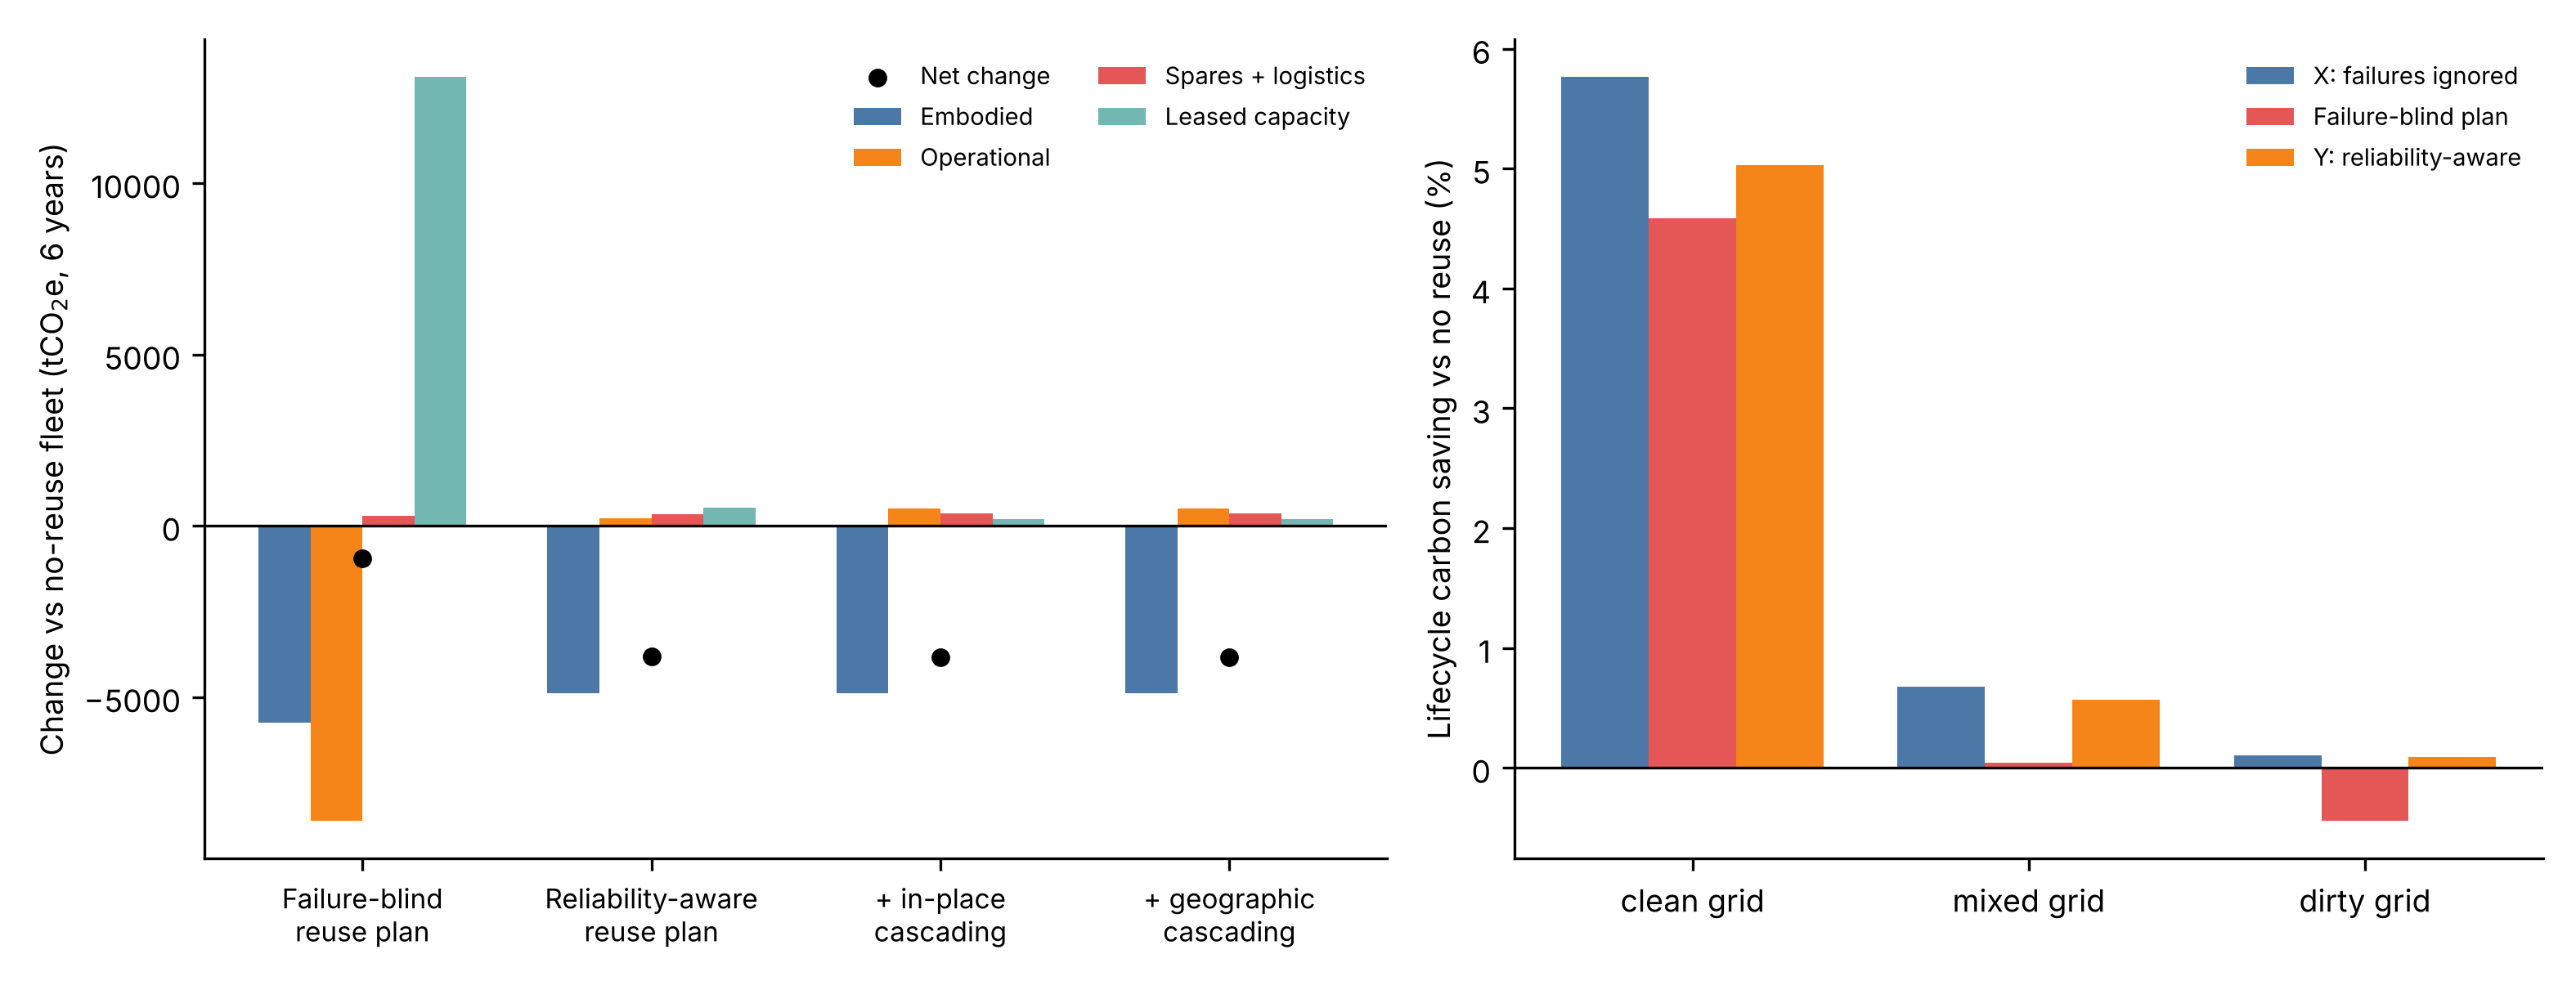
\includegraphics[width=0.80\linewidth]{figures/fig_fleet_carbon_ladder_by_grid.png}
\end{center}
\caption{Left: change in 6-year lifecycle carbon of the reference fleet relative to the no-reuse fleet (failures counted), by component, for the failure-blind plan, the reliability-aware plan, and the latter with in-place or geographic cascading; dots mark the net change. Right: $X$, failure-blind and reliability-aware savings for single-grid fleets. GPU throughput, power and CXL slowdown are placeholders.}
\label{fig:ladder}
\end{figure}

\begin{figure}[h]
\begin{center}
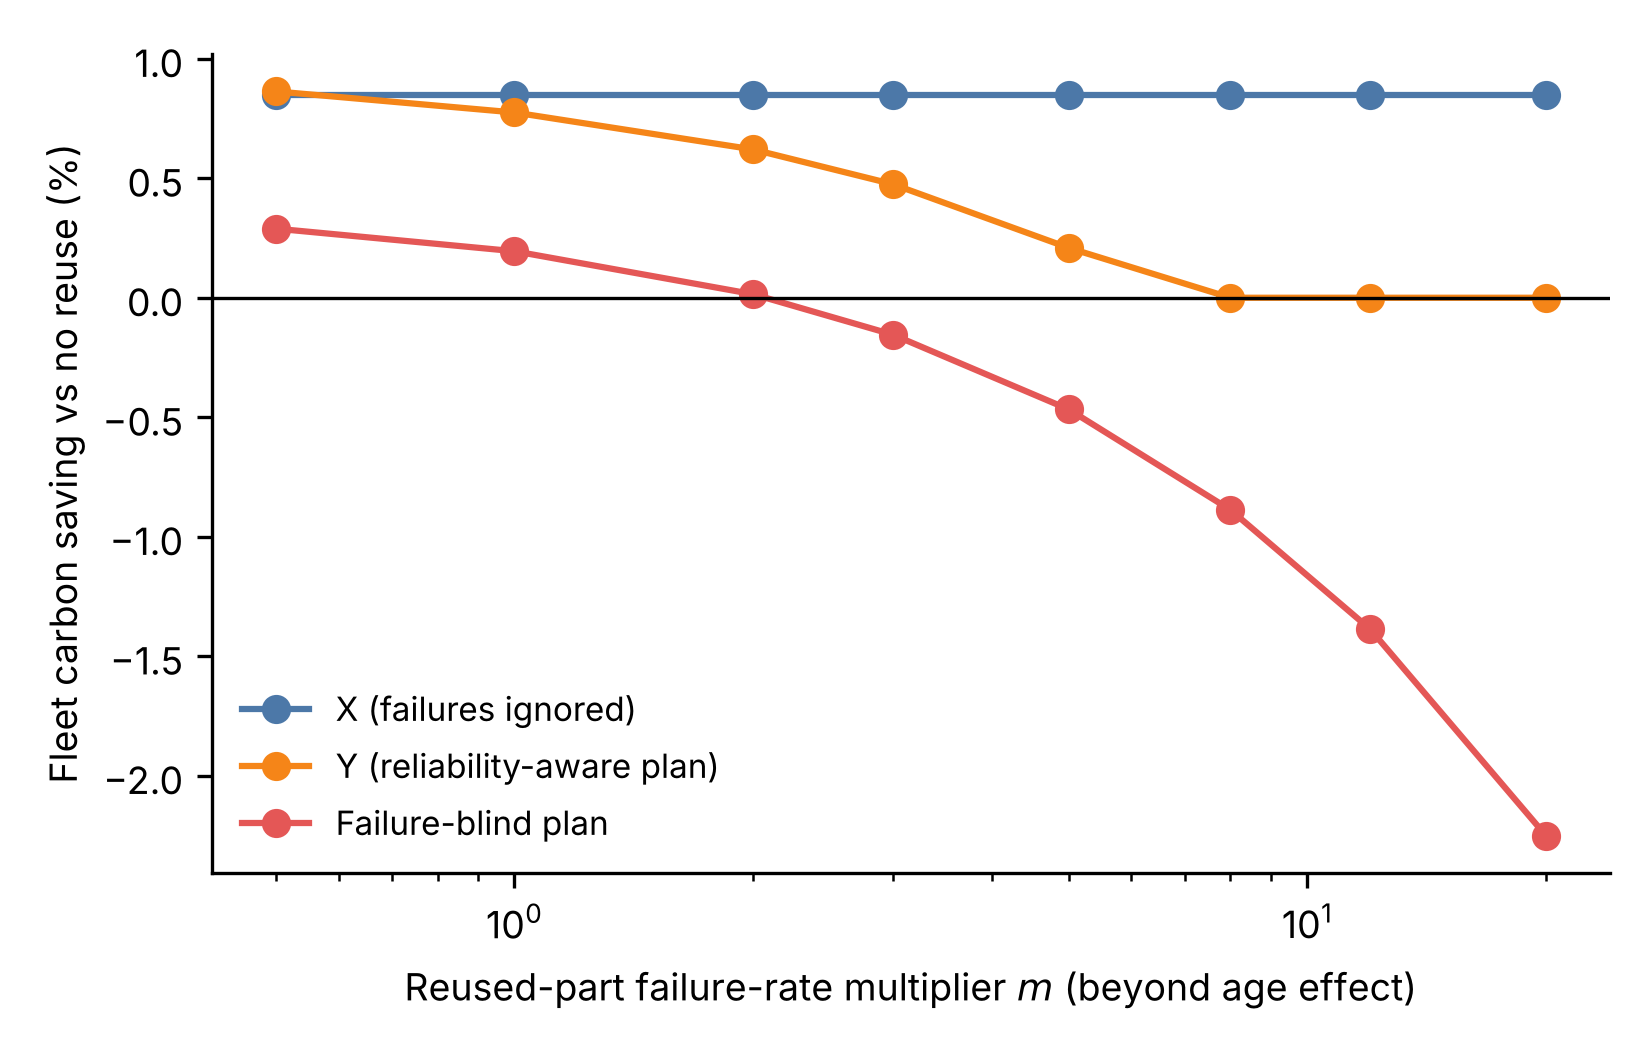
\includegraphics[width=0.44\linewidth]{figures/fig_reliability_breakeven_reused_parts.png}
\end{center}
\caption{Reference-fleet saving versus a multiplier $m$ on reused-part failure rates beyond the age effect (log scale). $X$ is flat; the reliability-aware plan still reuses at $m=5$ and has stopped by $m=8$ (no sweep points in between, so the crossover lies in $(5,8]$; it cannot do worse than no reuse by construction); the failure-blind plan crosses zero near $m \approx 2.1$ (interpolated), a value that mostly reflects the cost of ignoring drains (Section~\ref{sec:fleet}).}
\label{fig:breakeven}
\end{figure}

\begin{figure}[h]
\begin{center}
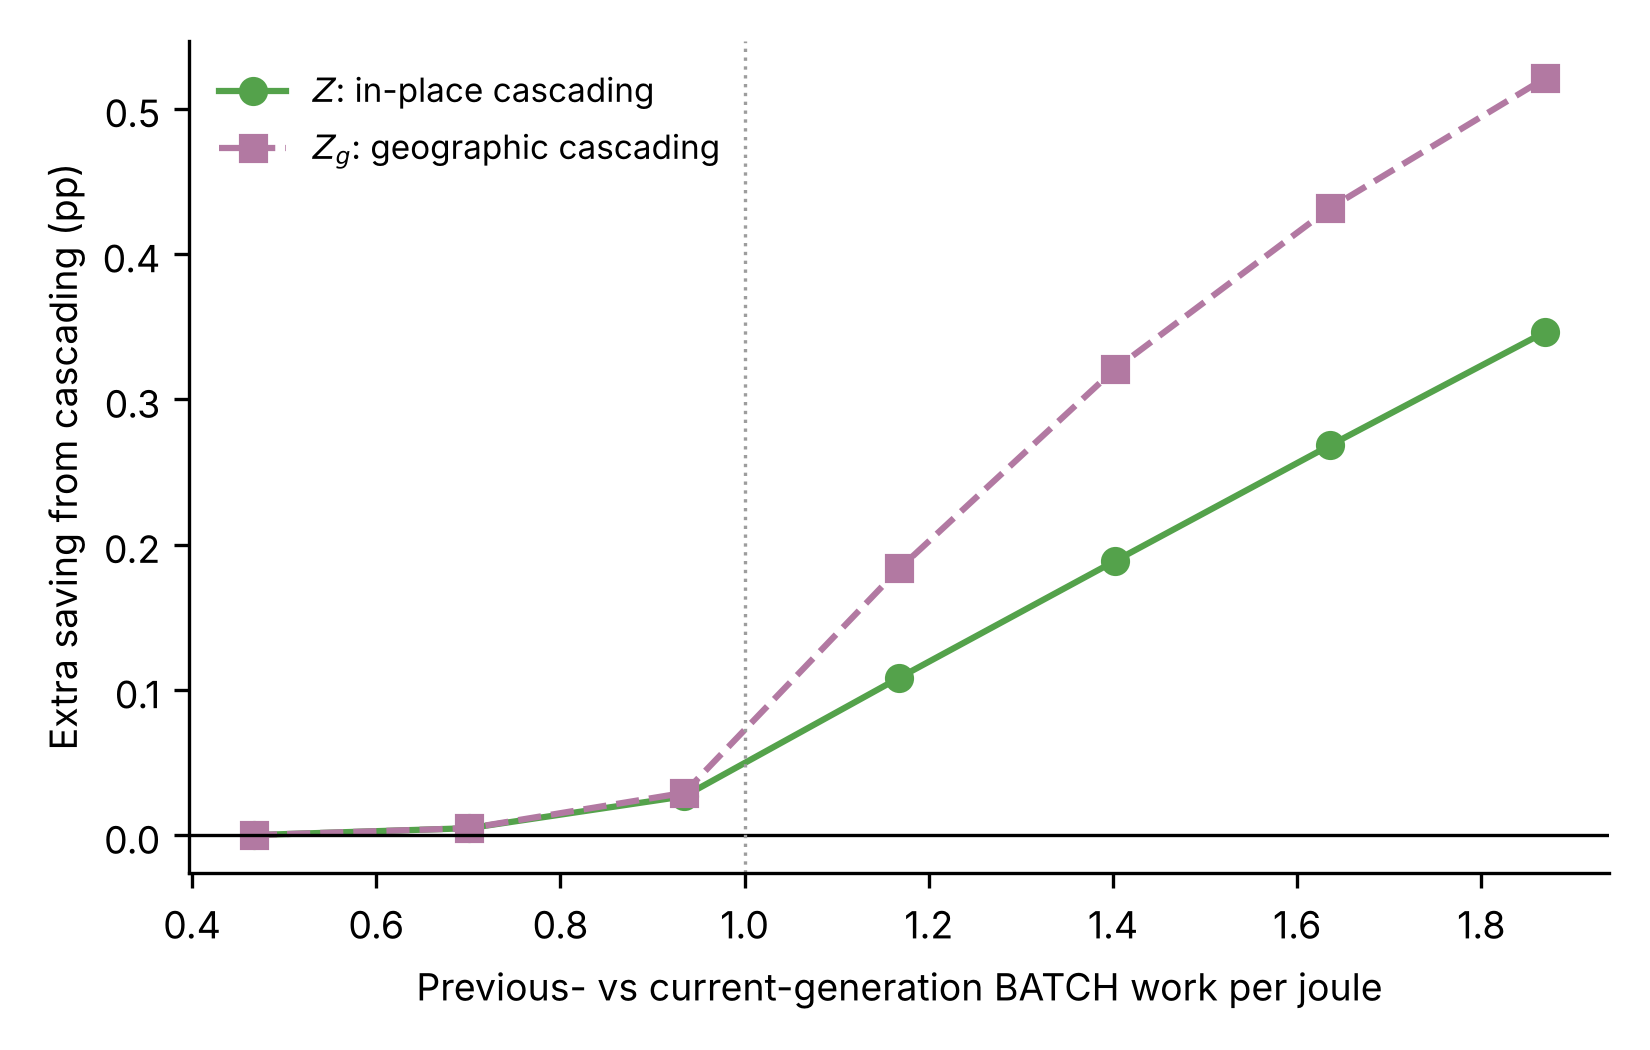
\includegraphics[width=0.46\linewidth]{figures/fig_cascade_breakeven_energy_efficiency.png}
\end{center}
\caption{Additional saving (pp) from cascading previous-generation GPU hosts to the batch tier versus their batch work per joule relative to current-generation hosts (dotted line: energy parity). $Z$: in-place; $Z_g$: geographic cascading to the clean-grid region. Cascading pays only near energy parity; geographic cascading adds further savings once cascading pays.}
\label{fig:cascade}
\end{figure}

\begin{figure}[h]
\begin{center}
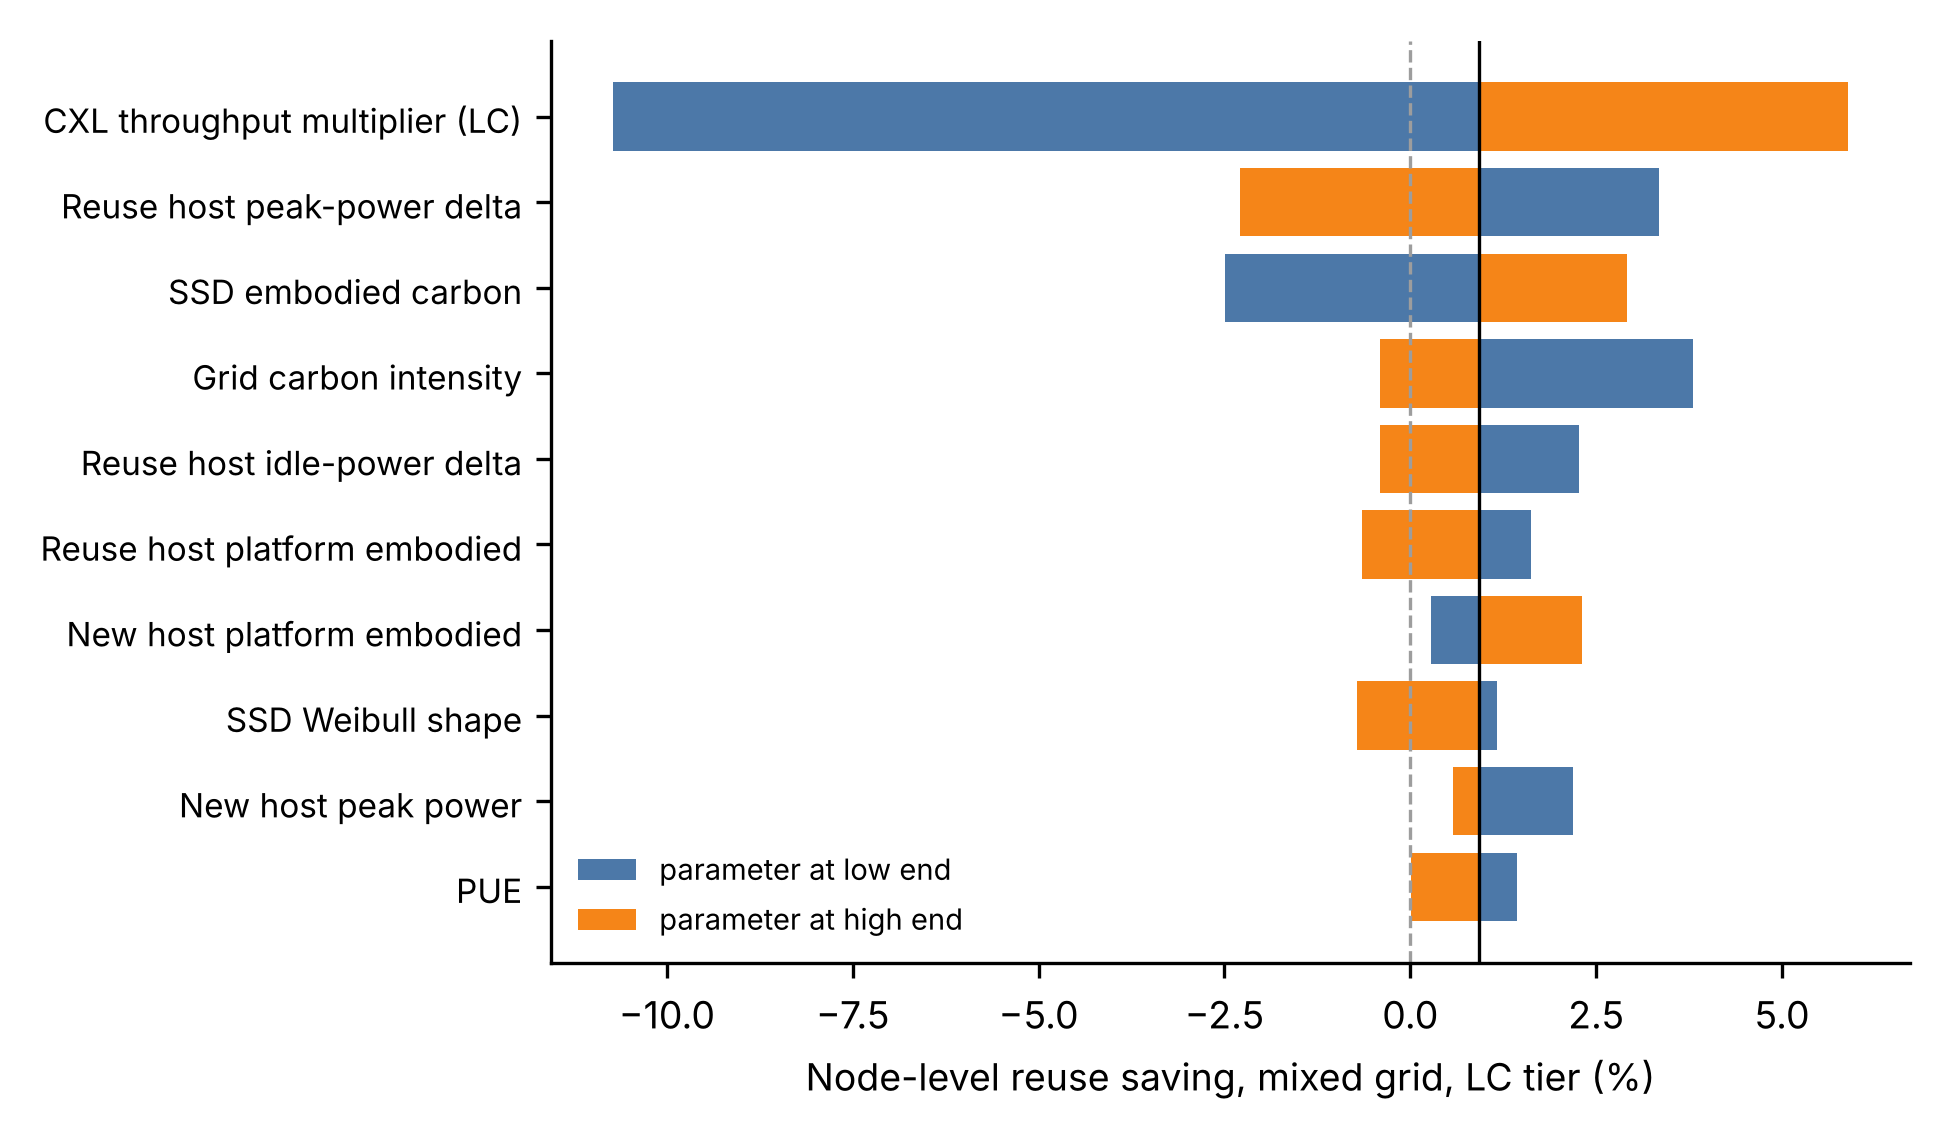
\includegraphics[width=0.56\linewidth]{figures/fig_node_sensitivity_tornado.png}
\end{center}
\caption{One-at-a-time sensitivity of the node-level reuse saving (mixed grid, LC tier). Bars start at the base saving (0.93\%, solid line) and show the saving with the parameter at the low (blue) and high (orange) end; the dashed line marks zero. The CXL throughput multiplier has by far the largest swing and is the dominant factor in the sign of the saving, but grid intensity and the reuse host's peak-power delta can also flip it within their ranges (Table~\ref{tab:breakeven}).}
\label{fig:tornado}
\end{figure}

\begin{figure}[h]
\begin{center}
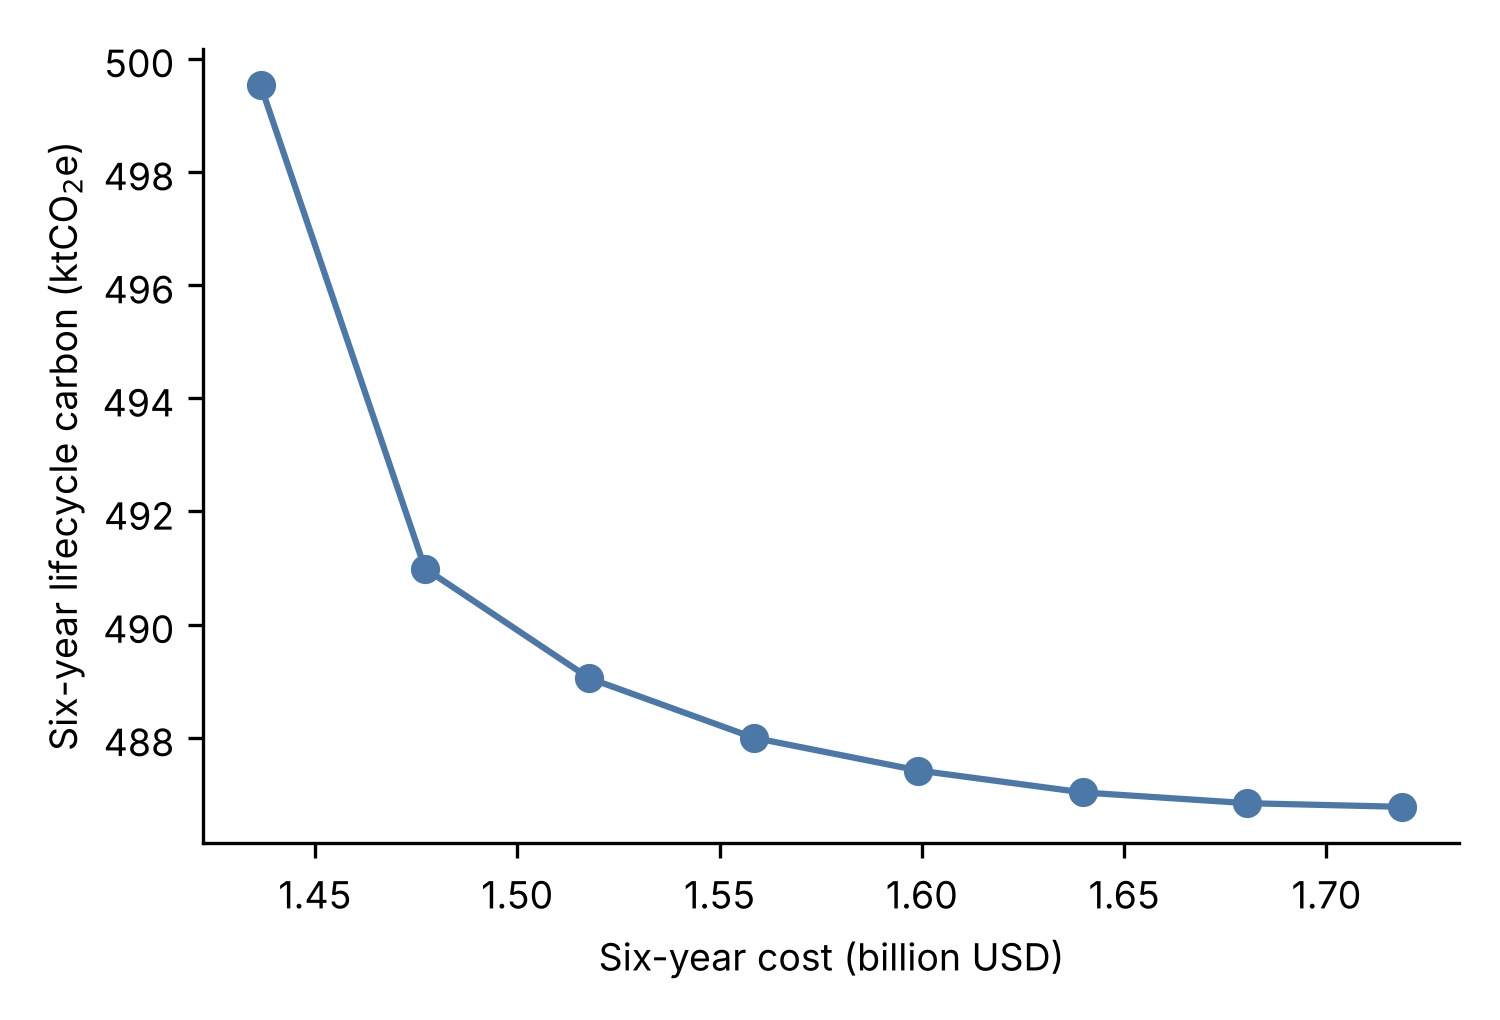
\includegraphics[width=0.42\linewidth]{figures/fig_carbon_cost_pareto.png}
\end{center}
\caption{Carbon-cost $\varepsilon$-constraint front of the reference fleet over six years (leftmost: cost-minimal plan; the logged rightmost endpoint has the same printed carbon as point 7 at higher cost, so point 7 is the carbon-minimal plan at printed precision).}
\label{fig:pareto}
\end{figure}

\section{Prepared Measurement Methodology}
\label{app:measure}
The following measurements have been prepared but \textbf{not executed}; no measured results are reported in this paper. (i) A \emph{serving benchmark} measures, per GPU generation, LC goodput at a time-to-first-token and time-per-output-token SLO and BATCH throughput, with board power sampled to obtain tokens per joule; it will replace the placeholder relative throughputs $\theta_{s\tau}$, the power parameters, and the old/new BATCH work-per-joule ratio that governs cascading. (ii) A \emph{KV-cache offload benchmark} measures decoding throughput with the KV cache in local versus remote-NUMA host memory as a proxy for CXL-attached reused DRAM; it will replace the placeholder CXL throughput multipliers (0.95 LC, 0.98 BATCH), the parameter with the largest sensitivity swing. Because emulated and real CXL memory can differ~\citep{Sun2023DemystifyingCxl}, this proxy will itself carry uncertainty. (iii) A \emph{KV-cache fault-injection study} flips bits in the KV cache at controlled bit-error rates under no protection, SECDED ECC, and block checksums with recomputation, to assess how errors in aged reused DRAM affect inference and which protection is needed.
%%%%%%%%% Appendix %%%%%%%%%

\end{document}